% Thesis format
\documentclass[11pt]{book}

%Select needed packages
\usepackage[paperwidth=17cm, paperheight=22.5cm, bottom=2.5cm, right=2.5cm]{geometry}
\usepackage{amssymb,amsmath,amsthm} 
\usepackage[spanish]{babel}
\usepackage[utf8]{inputenc} 
\usepackage{enumerate}
\usepackage{graphicx}
\usepackage[nottoc]{tocbibind}
\usepackage[pdftex,
            pdfauthor={NOMBRE DEL AUTOR},
            pdftitle={TÍTULO DE LA TESIS},
            pdfsubject={ÁREA DE LA TESIS},
            pdfkeywords={PALABRAS CLAVE},
            pdfproducer={Latex con hyperref},
            pdfcreator={pdflatex}]{hyperref}
\usepackage{natbib}
\usepackage[varg]{newtxmath}
\usepackage{newtxtext}
\usepackage{microtype}
\usepackage{xcolor}
\usepackage{fixltx2e}
\usepackage{booktabs}
\usepackage{siunitx}
\usepackage{color}
\usepackage{pdflscape}
\usepackage{rotating}
\usepackage{hyperref}
\usepackage[document]{ragged2e}

\hypersetup{colorlinks=True, linkcolor=blue!50!black, citecolor=black,
  urlcolor=blue!50!black}

\usepackage{etoolbox}
\robustify\bfseries
\robustify\itshape


%% Bold italic
\newcommand\hmmax{0}            % we don't need heavy fonts
\newcommand\bmmax{1}            % reduce use of math alphabets for bold
\usepackage{bm}

\usepackage{fancyhdr}

\pagestyle{fancy}
\fancyhf{}
\fancyhead[L]{\leftmark}
\fancyhead[R]{\rightmark}
\title{Tesis de doctorado\\
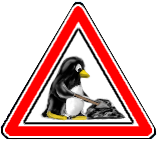
\includegraphics[width=0.1\linewidth]{./Figures/tux-development}
}

\author{Jorge Alejandro Tarango Yong}

\begin{document}
\maketitle
\begin{center}

\includegraphics[width=0.2\linewidth]{./Figures/logoUNAM}

\large
\textbf{UNIVERSIDAD NACIONAL AUTÓNOMA DE MÉXICO}

\rule{\linewidth}{0.1pt}

\rule[3mm]{0.7\linewidth}{1pt}


INSTITUTO DE RADIOASTRONOMÍA Y ASTROFÍSICA
\\[3\baselineskip]
``Estudio de la Interacción de Flujos Múltiples de Fuentes Astrofísicas, Aplicada
a los Proplyds Clásicos de la Nebulosa de Orión''
\\[2\baselineskip]

T E S I S
\\[2\baselineskip]
PARA OBTENER EL GRADO ACADÉMICO DE

DOCTOR EN CIENCIAS (ASTRONOMÍA)
\\[2\baselineskip]

P R E S E N T A
\\[2\baselineskip]
JORGE ALEJANDRO TARANGO YONG

Director de Tesis: Dr. William J. Henney
\\[2\baselineskip]
\normalsize
\end{center}
\begin{flushright}
Morelia, Michoacán

2017

\end{flushright}

\tableofcontents
\newpage
\section*{Agradecimientos}

Esta tesis se realizó para obtener el título de doctorado en 
ciencias (Astronomía). Deseo aprovechar esta sección para hacer
agradecimientos a personas y/o instituciones que me ayudaron para que 
pueda completar este trabajo de manera exitosa.
\newpage
\section*{Resumen}
  Abstract en español

\newpage
\section*{Abstract}
  Abstract written in english

\newpage
\chapter{Objetos Astrofísicos Relevantes}
\section{La Nebulosa de Orión}
\section{Estrellas ``Errantes''}
\section{Discos Protoplanetarios}
\section{Proplyds}
\subsection{Descubrimiento}
Observaciones en óptico de la región del trapecio en filtros de banda
angosta de diferentes líneas de emisión tales como $H\alpha$, $H\beta$,
$[OIII]$, $[NII]$, $[SII]$ y continuo, revelaron la existencia de
objetos puntuales únicamente visibles en líneas de alta ionización
($H\alpha$, $H\beta$ y $[OIII]$) que fueron inicialmente denominados como
``condensaciones nebulares'' \citep{Laques:1979}. 

Hasta el momento no se sabía con certeza si ``condensaciones nebulares''
eran en realidad condensaciones nebulares (regiones donde la densidad de
la nebulosa es inusualmente alta por alguna razón o bien esferas de gas
molecular cuya envolvente fue ionizada y que la radiación de la estrella
central la está ``erosionando'') o si se trataba de protoestrellas
de baja masa cuyo disco protoplanetario estaba siendo fotoevaporado por
la estrella central \citep{churchwell:1987}. No fue sino hasta que se contó
con observaciones de alta resolución con el Telescopio Espacial Hubble (HST)
que se se pudo determinar la verdadera naturaleza de estos objetos
\citep{ODell:1993} y la razón por la que se les denominó ``proplyds''
(PROtoPLanetarY DiskS). A su vez se encontraron por primera vez arcos
delgados y otras estructuras de gran interés.

\subsection{¿Qué es un proplyd? Breve introducción}

\subsection{Mecanismos de fotoevaporación \citep{Johnstone:1998}}

El principal mecanismo de fotoevaporación es el campo de radiación de la
estrella central, especialmente en la parte ultravioleta del espectro
electromagnético. Según la masa de la estrella central, podemos tener dos
clases de flujo radiativo: Dominado por el ultravioleta lejano (FUV,
$h\nu < 13.6~eV$) o dominado por el ultravioleta extremo (EUV,
$h\nu \geq 13.6~eV$). En general, el FUV se encarga de disociar moléculas
y de calentar el gas de la región de fotodisociación (PDR) hasta
temperaturas de 100 - 1000 K, mientras que el EUV puede ionizar el gas y
elevar su temperatura hasta $10^4~K$. El EUV no puede atravesar el frente
de ionización (IF) pero el FUV sí.

En el caso de que el flujo sea dominado por el EUV, la presión térmica del
flujo fotoevaporado es determinada por la fotoionización, la PDR producida
por el FUV es delgada. El gas calentado por el FUV se mueve de manera
subsónica hasta llegar al IF y la tasa de pérdida de masa
depende de la tasa de ionización inducida por el EUV.

Si el flujo está dominado por el FUV, la presión térmica depende del
calentamiento por el FUV. El gas tibio se expande como un viento que empuja
el IF lejos del disco. La tasa de pérdida de masa la determina la temperatura
de la PDR, el flujo FUV y la opacidad del polvo a las longitudes de onda del FUV.

Inicialmente la forma del disco impone una geometría cilíndrica en el
flujo fotoevaporado, pero eventualmente los gradiente de presión tornan
esta geometría en esférica.

Las ecuaciones de continuidad de la masa y el momento restringen la velocidad
del flujo neutro antes de alcanzar el IF. Mas allá de éste, la presión del
gas hace que éste se expanda a velocidades del orden de una a dos veces la
velocidad del sonido. Para el gas neutro dentro del IF hay dos posibles
soluciones: si el gas neutro es supersónico entonces el IF será de baja
densidad (Tipo R) con bajo contraste de densidad entre gas neutro y
gas ionizado. O si el gas neutro es subsónico se formará un IF tipo D con un
gran contraste de densidad entre el gas neutro y el gas ionizado. Sin embargo,
sin importar qué tipo de radiación domina la fotoevaporación, el gas neutro
permanece a velocidades subsónicas al llegar al IF, por lo que dicho frente
será tipo D. 
En el caso de un flujo dominado por el EUV, el gas neutro permanece a
velocidad subsónica, su velocidad decae como $v_I \prop r^{-2}$ y llega
a $0.5~kms^{-1}$ al llegar al frente de ionización. Cundo el flujo es
dominado por el FUV, el gas neutro se acelera hasta llegar a velocidades
supersónicas, luego atraviesa un choque isotérmico que lo desacelera y
llega al frente de ionizacion a $0.5~kms^{-1]$.

  \begin{figure}
    \begin{tabular}{cc}
      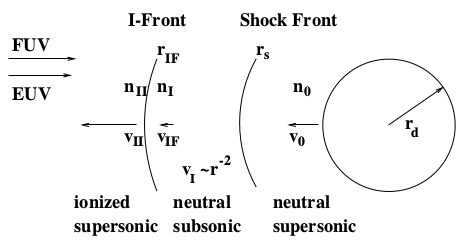
\includegraphics[width=0.5\linewidth]{./Figures/Johnstone-2} &
      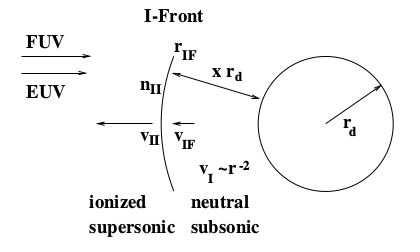
\includegraphics[width=0.5\linewidth]{./Figures/Johnstone-3}
    \end{tabular}
    \label{fig:EUV-FUV-IF}
    \caption{Representación esquemática de las regiones del flujo
      fotoevaporado de un proplyd. Izquierda: Cuando el flujo es dominado
    por el FUV. Derecha: Flujo dominado por EUV \citep{Johnstone:1998}}
  \end{figure}
  

Sin importar el tipo de mecanismo de fotoevaporación dominante, el flujo
fotoevaporado solo si la presión térmica supera a la gravedad de la
protoestrella. Entonces, el flujo fotoevaporado solo existe a partir de
un radio crítico $r_g$, donde este radio se estima a partir del balance
entre la energía necesaria para escapar de una órbita kepleriana y la
energía térmica:
\begin{align}
  r_g = \frac{GM_*}{a^2}
\end{align}
Donde $M_*$ es la masa de la protoestrella y $a$ es la velocidad del sonido
del gas. Para las protoestrellas típicas del trapecio la masa típica es de
$M_* = 0.2~M_\odot$. Para el gas neutro la velocidad del sonido es de
$a_I \sim 3~km~s^{-1}$ y para el gas ionizado es de $a_{II} \sim 10~km~s^{-1}$.
Por tanto, el radio gravitacional para un flujo dominado por el EUV es de
$r_{gII} \sim 2~AU$ y para un flujo dominado por el FUV es de
$r_{gI} \sim 20~AU$. El radio del frente de ionización escala como
$r_{IF} \prop D^{2/3}$

\subsection{Forma del frente de ionización \citep{Johnstone:1998}}





\section{Objetos LL}
\subsection{Mapa de Objetos}
\chapter{Marco Teórico}
\chapter{Marco Teórico}
\section{Vientos Estelares}
\section{Choques}
\section{Frentes de Ionización}
Un frente de ionización es la interfaz entre un medio gaseoso neutro y uno
ionizado. Ocurren cerca de fuentes de rediación ionizante, tales como
estrellas masivas, tipo B temprana o tipo O. el frente de ionización puede
tratarse como una discontinuidad en el medio gaseoso.

\section{Regiones HII \citep{Stahler:2004}}
\label{sec:HII}
\newcommand\Nio{\ensuremath{\mathcal{N}}}
%\newcommand\N{\ensuremath{\mathcal{N}}}

Consideremos el caso en que se forma una estrella masiva dentro de una nube molecular, que por simplicidad está compuesta exclusivamente de hidrógeno molecular $H_2$. La estrella masiva emite fotones ultravioleta que tienen la energía suficiente para disociar el $H_2$  como para ionizar el hidrógeno atómico resultante. Luego el plasma ionizado se recombina para volver a ser $HI$ emitiendo líneas espectrales de diversas energías, siendo la más energética la línea de $\mathrm{Ly~}\alpha$. Como al realizar una ionización se pierde un fotón ionizante y el flujo de radiación proveniente de la estrella es finito, entonces la estrella solo puede ionizar la región de la nube más próxima a ésta. Si suponemos que la nube tiene densidad uniforme, entonces esta región tendrá forma esférica, conocida como \textit{esfera de Strömgren}.

\subsection{Esfera de Strömgren}

El plasma ionizado dentro de la Esfera de Strömgren se encuentra en balance de ionización, esto es, que la tasas de ionización y la de recombinación son iguales. La tasa de ionizaciones es igual a la cantidad de fotones ionizantes que emite la estrella central por segundo. Esto es, los fotones que poseen una energía mayor al límite de Lymann, que corresponde a  $E = 13.6\mathrm{~eV}$, o bien $\lambda = 912\mathrm{~\AA}$. En la tabla \ref{tab:ionizing-radiation} se muestra la tasa de fotones ionizantes $\Nio_*$ para estrellas masivas de tipo espectral O y B temprano.

\begin{table}
  \begin{tabular}{cccc} \hline 
    Tipo & Masa & $\log \Nio_*$ & \log \Nio_{FUV} \\
    Espectral & $(M_\odot)$ & $(s^{-1})$ & $(s^{-1})$  \\
    \hline
    O4 & 70 & 49.9 & 49.5 \\
    O5 & 60 & 49.4 & 49.2 \\
    O6 & 40 & 48.8 & 48.8 \\
    O7 & 30 & 48.5 & 48.6 \\
    O8 & 23 & 48.2 & 48.4 \\
    O9 & 20 & 47.8 & 48.2 \\
    B0 & 18 & 47.1 & 48.1 \\
    B1 & 13 & 45.4 & 47.5 \\
    B2 & 10 & 44.8 & 47.1 \\
    \hline
  \end{tabular}
  \caption{Tasa de fotones ionizantes para estrellas masivas \citep{Stahler:2004}}
  \label{tab:ionizing-radiation}
\end{table}

Por otro lado, la tasa volumétrica de recombinaciones se escribe como:

\begin{align}
  \ensuremath{\mathcal{R}} = n_e n_p \alpha_{rec}(T) = n^2_e \alpha_{rec}(T)
\end{align}

Donde $\alpha_{rec}$ es el \texit{coeficiente de recombinación}, y es una función solo de la temperatura. La última iguladad se obtiene asumiendo neutralidad de la carga.

La tasa total de recombinaciones se obtiene integrando $\ensuremath{\mathcal{R}}$ en el volumen de la región $HII$, asumiendo que tanto la densidad de electrones como la tempertaura son constantes espacialmente. De esta manera la condición de balance de ionización queda como sigue:

\begin{align}
  \Nio_* = \frac{4\pi}{3} n^2_e \alpha'_{rec}(T)R^3_s 
\end{align}

Donde $R_s$ es el \textit{radio de Strömgren}. Es importante notar que el coeficiente de recombinación primado es diferente del coeficiente no primado: el coeficiente de recombinación primado no toma en cuenta las recombinaciones al nivel $n = 1$ debido a que estas recombinaciones producen fotones de $E = 13.6\mathrm{~eV}$ que son capaces de ionizar el hidrógeno neutro.

Como la densidad de la nube original no cambia apreciablemente cuando el gas es ionizado debido a que el tiempo en que esto pasa es muy corto (como mostraremos en la siguiente sección), entonces $n_e = n^0_H$, donde $n^0_H$ es la densidad de $HI$ en la región contigua a la nube, y a su vez $n^0_H = n_{H_2}$, donde $n_{H_2}$ es la densidad de gas molecular. Con esto podemos calcular el radio de Strömgren como sigue:

\begin{align}
  R_s = \left[\frac{3\Nio_*}{4\pi\alpha'_{rec}(n^0_H)^2}\right]^{1/3} = 0.4\mathrm{~pc}\left(\frac{\Nio_*}{10^{49}\mathrm{~s^{-1}}}\right)^{1/3}\left(n_{H_2}\right)^{-2/3}
\end{align}

En la expresión numérica, se adopta un valor de $\Nio_*$ de $10^{49}\mathrm{s^{-1}}$, una temperatura de $10^4\mathrm{~K}$ que es la temperatura característica de una región $HII$ y con la que el coeficiente de recombinación $\alpha'_{rec}$ adopta un valor de $2.6\times 10^{-13}\mathrm{~cm^3~s^{-1}}$.

Dentro de la región $HII$, la probabilidad por unidad de tiempo de ionizar un átomo de hidrógeno dado es mucho mayor a la probabilidad de una recombinación, por lo que el gas está casi completamente ionizado. Sin embargo, en los bordes de la región $HII$, la densidad de gas neutro aumenta debido a que en dicha región el flujo de fotones ionizantes ha sido atenuado por todo el gas ionizado más próximo a la estrella. La transición de gas ionizado a gas neutro tiene un grosor $\Delta r$ que corresponde al camino libre medio del gas neutro. Esto es:

\begin{align}
\Delta R = \frac{1}{\sigma_{\nu_1}n^0_H}  
\end{align}

Donde $\sigma_{\nu_1}$ es la sección recta de un átomo de hidrógeno en el estado base, evaluada en la longitud de onda del límite de Lymann. Utilizando $\sigma_{\nu_1} = 6.8\times 10^{-18}\mathrm{~cm^2}$ y $n^0_H = 2\times 10^{3}\mathrm{~cm^{-3}}$ obtenemos que $\Delta r = 7.4\times 10^{13}\mathrm{~cm} \sim 5\times 10^{-5}~R_s$, lo que muestra que las regiones $HII$ tienden a tener bordes bien delimitados.

\subsection{Primera y Segunda expansión}

Las esferas de Strömgren no son objetos estáticos, sino que se expanden con el tiempo. Este proceso ocurre en dos etapas: en la primera inicialmente no existe ninguna región $HII$ pero que la radiación ultravioleta de la estrella hace que se expanda rápidamente al disociar e ionizar el gas a su alrededor hasta alcanzar el radio de Strömgren. En la segunda expansión la diferencia de presiones entre el gas ionizado de la región $HII$, mucho mayor que la del gas neutro que lo rodea, provoca otra expansión más lenta que la primera hasta que haya equilibrio de presión. A continuación explicaremos el proceso más a detalle:

Sea $F_*(t)$ el flujo de radiación ionizante que alcanza un radio $R$ al tiempo $t$. Al transcurrir un tiempo $dt$, el frente de ionización avanza una distancia $dR$ y llega a $n^0_{H_2}$ moléculas de hidrógeno por unidad de área. Se necesitan 3 fotones para ionizar completamente la molécula: uno para disociarla, con energía $E\geq 14.7\mathrm{~eV}$ y otros dos para ionizar cada uno de los átomos resultantes, con $E\geq13.6\mathrm{~eV}$. El número de fotones ionizantes atravezando el frente de ionización por unidad de área es $F_*~dt$. Entonces, como se producen dos ionizaciones por cada tres fotones, tenemos que:

\begin{align}
  \frac{F_* dt}{2 n_{H_2} dR} &= \frac{3}{2} \\
  \implies \frac{dR}{dt} &= \frac{F_*}{3n_{H_2}} = \frac{2 F_*}{3 n^0_H}
\end{align}

Estamos asumiendo que el flujo tanto de fotones con energías de $E\geq 14.7\mathrm{~eV}$ y $E\geq 13.6\mathrm{~eV}$ es prácticamente el mismo.

Ahora consideremos las recombinaciones: el número total de recombinaciones que llevan a niveles tales que $n \geq 2$ dentro de una esfera de radio $R$ es $\frac{4\pi}{3}\left(n^0_H\right)^2\alpha'_{rec}R^3$. Si el balance de ionización aun se mantiene, entonces el número de ionizaciones por unidad de tiempo es igual a la tasa de recombinaciones más los fotones que logran atravesar el frente de ionización por unidad de tiempo que es $4\pi R^2 F_*$. Entonces:

\begin{align}
  \Nio_* = 4\pi R^2 F_* + \frac{4\pi}{3}\left(n^0_H\right)^2\alpha'_{rec}R^3
\end{align}

Resolvemos para $F_*$ y encontramos que:

\begin{align}
  F_* &= \frac{\Nio_*}{4\pi R^2} - \frac{\left(n^0_H\right)^2\alpha'_{rec} R}{3} \\
  \implies \frac{dR}{dt} &= \frac{\Nio_*}{6\pi n^0_H R^2} - \frac{2n^0_H \alpha'_{rec} R}{9} \label{eq:1-expansion-eq} 
\end{align}

Definimos los siguientes parámetros adimensionales $\lambda \equiv R/R_s$ y $\tau \equiv t/t_{rec}$, donde $t_{rec} = \frac{1}{n^0_H \alpha'_{rec}}$ es el tiempo medio de recombinación del hidrógeno, que es del órden de $60\mathrm{~yr}$ con los valores de $n^0_H$ y $\alpha'_{rec}$ utilizados en esta sección. Y con esto la ecuación (\ref{eq:1-expansion-eq}) se escribe como sigue:

\begin{align}
  \frac{d\lambda}{d\tau} = \frac{2}{9}\left(\lambda^{-2} - \lambda\right)
\end{align}

Resolvemos por el método de separación de variables y aplicamos la condición inicial $\lambda(0) = 0$ y obtenemos lo siguiente:

\begin{align}
  \lambda(\tau) = \left[1 - \exp\left(-\frac{2}{3}\tau\right)\right]^{1/3} \label{eq:lambda-tau}
\end{align}

De la ecuación (\ref{eq:lambda-tau}) vemos que cuando han pasado dos terceras partes del tiempo de recombinación,  la región $HII$ se ha expandido alrededor del $86\mathrm{\%}$ del radio de Strömgren, y aunque la expansión se va descelerando constantemente, ya es de una extensión considerable.

\subsection{Flujos de Champaña}
\subsection{Características de la emisión}
% Las regiones HII se forman cuando una estrella masiva, de tipo espectral O ó B temprana, ioniza el gas que se encuentra a su alrededor. El gas ionizado se encuentra en equilibrio térmico, a una temperatura del orden de $10^4~\mathrm{K}$. El principal proceso de calentamiento es la radiación de la estrella central, mientras que el enfriamiento se da principalmente por la recombinación de líneas prohibidas y por emisión libre-libre.

\section{Modelo Genérico de los Choques de Proa}
\label{sec:Modelo-generico}
Para este trabajo consideramos en general dos modelos de
interacción  de vientos:
\begin{itemize}
\item Una fuente localizada en el origen que emite un viento esférico
  que puede ser isotrópico o anisotrópico (figura
  \ref{fig:isotropic-aniso}) no acelerado que interactúa con el viento
  esférico isotrópico de otra fuente que se encuentra a una distancia
  $D$ de la primera(figura \ref{fig:crw-esquema})
\item Una fuente localizada en el origen que emite un viento esférico
  isotrópico no acelerado que interactúa con un viento plano paralelo
  no acelerado y densidad constante (figura )
\end{itemize}
El sitema en su conjunto tiene simetría cilíndrica.
\begin{figure}
  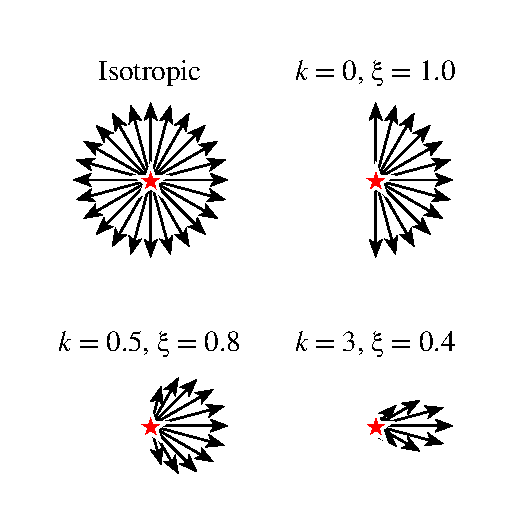
\includegraphics[width=0.5\linewidth]{./Figures/anisotropic-arrows}
  \caption{Representación esquemática de vientos con diferentes
    anisotropías:
    Arriba izquierda: Viento isotrópico esférico. Arriba derecha: viento
    isotrópico hemisférico. Abajo: Vientos anisotrópicos donde el
    parámetro $k$ indica el grado de anisotropía (ver capítulo \ref{chap:hipersonica})}
    \label{fig:isotropic-aniso}
\end{figure}
\begin{figure}
  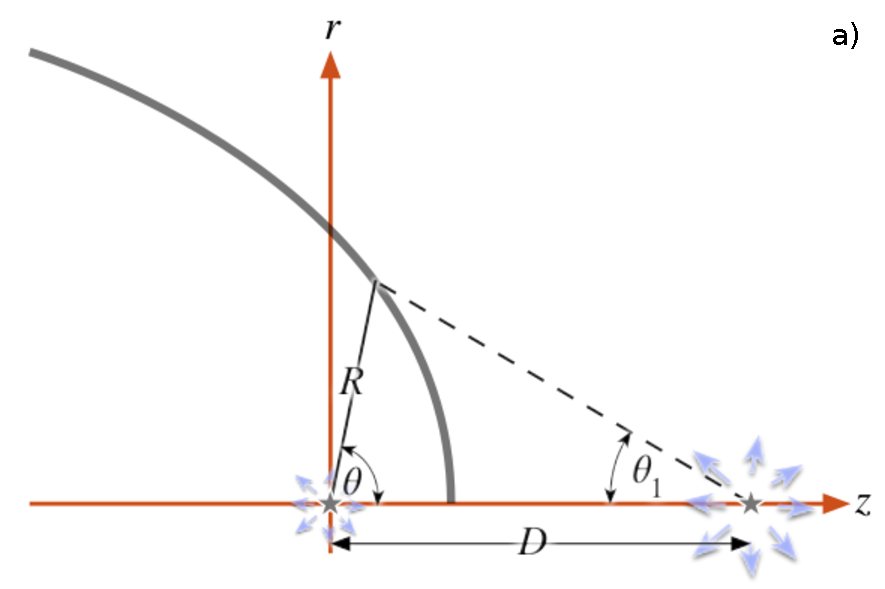
\includegraphics[width=0.5\linewidth]{./Figures/bowshock-crw-variables}
  \caption{Representación esquemática del problema de interacción de dos vientos:
    Dos fuentes separadas por una distancia $D$ emiten un viento radial que forma un
    choque de proa a una distancia $R$ del origen. El sistema tiene geometría cilíndrica
    siendo el eje $z$ el eje de simetría. La forma del choque depende únicamente del ángulo
    polar $\theta$, medido a partir del origen. Otro ángulo que es de utilidad es $\theta_1$,
    que corresponde al ángulo polar medido a partir de la posición de la otra fuente.}
    \label{fig:crw-esquema}
\end{figure}

\subsection{Planitud y ``Alatud''}
\label{sec:char-rad}
Las cantidades medibles que nos ayudan a caracterizar un choque de proa las
llamamos ``Radios característicos'' (ilustrados en la figura
\ref{fig:char-radii}):
\begin{itemize}
\item Radio del choque en la dirección del eje de simetría del sistema.
  Denotado como $R_0$
\item Radio en dirección perpendicular al eje de simetría del sistema.
  Denotado como $R_{90}$
\item Radio de curvatura en la ``nariz'' del choque de proa. Denotado
  como $R_c$. En el apéndice \ref{app:math-curvature-radius} se muestra
  el procedimiento para obtener este radio para una curva genérica continua
  y derivable.
\end{itemize}

\begin{figure}
  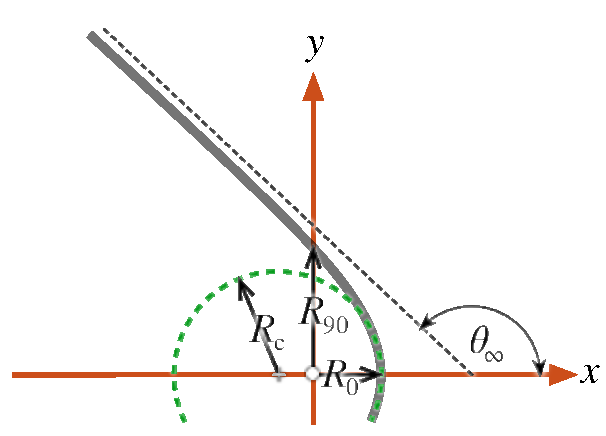
\includegraphics[width=0.5\linewidth]{./Figures/characteristic-radii}
  \caption{Representación esquemática de los radios característicos
    de un choque de proa}
  \label{fig:char-radii}
\end{figure}
Un último parámetro es el ángulo asintótico de apertura de las alas, denotado como $\theta_\infty$. Sin embargo, en la mayoría de los choques de proa es dificil de medirlo debido a que el ángulo polar $\theta$ tiende al valor asintótico muy lentamente y además la emisión de las alas es bastante débil. Por otro lado, los radios característicos $(R_0, R_c, R_{90})$ son medibles observacionalmente en la mayoría de los casos. A partir de éstos, podemos determinar dos parámetros adimensionales llamados ``planitud'' y ``alatud''. El primero de éstos es una medida de qué tan plano es el choque de proa en la nariz o ``apex'', y lo denotamos con la letra griega $\Pi$, mientras que el segundo es una medida de qué tanto se abren las alas del choque de proa, y lo denotamos con la letra griega $\Lambda$. Ambos parámetros se definen a continuación:

\begin{align}
  \Pi \equiv \frac{R_c}{R_0} \\
  \Lambda \equiv \frac{R_{90}}{R_0}
\end{align}

  
%Para este trabajo resulta útil hacer una noramlización de los radios
%característicos u otros radios, para que las mediciones que obtengamos
%sean adimensionales. De esta forma, podemos hacer la normalización con
%la distancia $D$, o bien con $R_0$, dependiendo de qué tipo de
%normalización resulte más conveniente. En el primer caso expresamos
%explícitamente el cociente (e.g $\frac{R_0}{D}$, $\frac{R_c}{D}$,
%$\frac{R_{90}}{D}$), y en el segundo caso añadiremos una tilde al
%radio en cuestión (e.g $\tilde{R}_c$, $\tilde{R}_{90}$). 

\section{Proyección en el Plano del Cielo}
\label{sec:projection}

Para un choque de proa que es la vez geométricamente delgado y
ópticamente delgado, únicamente se observa el borde de éste por
abrillantamiento al limbo, por lo tanto, su orientación respecto a
la línea de visión modifica su forma respecto a la forma real del
choque. Para ello, rotamos el sistema de referencia del choque de proa
en coordenadas cartesianas, denotado por $(x, y, z)$, por un ángulo
que llamamos \textit{inclinación}, denotado por $i$, en el plano $xz$,
de modo que la transformación entre el sistema de refencia del choque
y el sistema de referencia del plano del cielo, denotado por
$(x', y', z')$ queda como sigue:

\begin{align}
  \left(
  \begin{array}{c}
    x' \\ y' \\ z'
  \end{array}
  \right) &=
  \left(
  \begin{array}{c}
    x\cos i - z\sin i \\ y' \\ z\cos i + x\sin i
  \end{array}
  \right)
  \label{eq:rotation}
\end{align}

Por otro lado, la forma tridimensional del choque de proa viene dado por:

\begin{align}
  \left(
  \begin{array}{c}
    x \\ y \\ z
  \end{array}
  \right) &=
            R(\theta)\left(
            \begin{array}{c}
              \cos\theta \\
              \sin\theta\cos\phi \\
              \sin\theta\sin\phi
            \end{array}
            \right)
\end{align}
La relación entre ambos sistemas de referencia se ilustra en la figura
\ref{fig:reference}.

\begin{figure}
  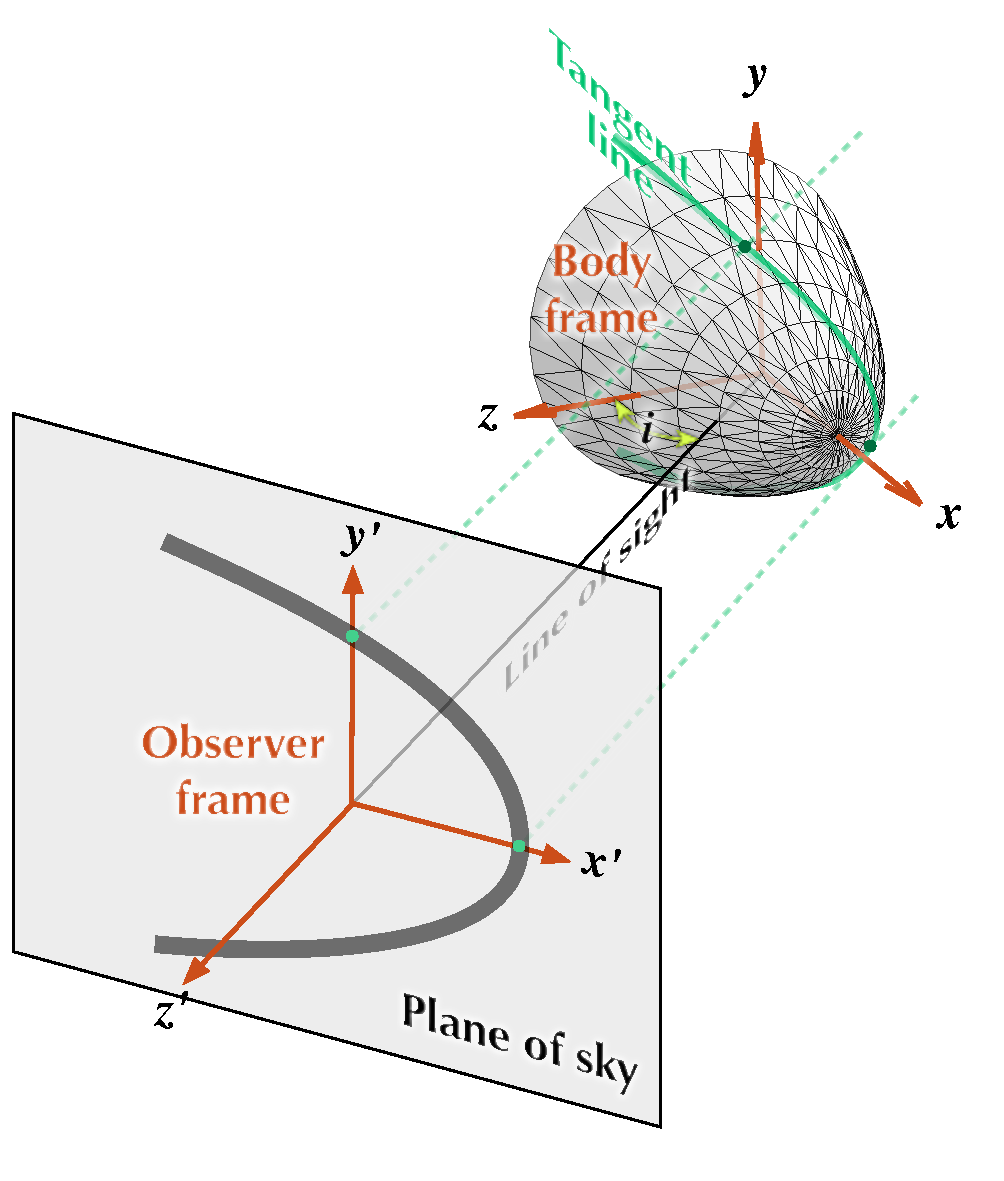
\includegraphics[width=0.5\linewidth]{./Figures/projection-pos}
  \label{fig:reference}
  \caption{Sistema de referencia del choque vs sistema de referencia del
    plano del cielo. Los ejes $x'$ y $y'$ se encuentran en el plano del
    cielo, mientras el eje $z'$ es paralelo a la línea de visión.
    Solo la regi\'on del choque cuya tangente sea paralela a la l\'inea
    de visión será visible por abrillantamiento al limbo.}
\end{figure}

\subsection{Vectores normal y tangente a la superficie}

Si definimos los vectores $\hat{n}$ y $\hat{t}$, como los vectores
normal y tangente a la superficie, respectivamente para $\phi$ constante.
En el caso $\phi = 0$ (figura \ref{fig:unit-vec}), ambos vectores se encuentran
en el plano $xy$ y es fácil mostrar que:

\begin{align}
  \hat{t}_0 =
  \left(
  \begin{array}{c}
    -\cos\alpha \\
    \sin\alpha \\
    0
  \end{array}
  \right)
  \quad \mathrm{y} \quad
  \hat{n}_0 =
  \left(
  \begin{array}{c}
    \sin\alpha \\
    \cos\alpha \\
    0
  \end{array}
  \right)
  \label{eq:unit-vec}
\end{align}

Donde:
\begin{align}
  \tan\alpha = -\frac{dy}{dx} = \frac{1+\omega\tan\theta}{\tan\theta-\omega}
\end{align}
y:
\begin{align}
  \omega(\theta) = -\frac{1}{R}\frac{dR}{d\theta} 
\end{align}

Para otros valores de $\phi$, basta con hacer una rotación de las ecuaciones
(\ref{eq:unit-vec}) alrededor del eje $x$. Para la conversión al sistema de
referencia del plano del cielo se utiliza la ecuación (\ref{eq:rotation}):

\begin{align}
\begin{split}
  \hat{n}' &= \frac{1}{\left(1 + \omega^2\right)^{1/2}} \\
           & \times \left(
             \begin{array}{c}
               (\cos\theta+\omega\sin\theta)\cos i-(\sin\theta-\omega\cos\theta)\sin i\sin\phi\\
               (\sin\theta-\omega\cos\theta)\cos\phi \\
               (\cos\theta+\omega\sin\theta)\sin i+(\sin\theta-\omega\cos\theta)\sin\phi\cos i
             \end{array}
                    \right) \\
\end{split}\\
\begin{split}
    \hat{t}' &= \frac{1}{\left(1 + \omega^2\right)^{1/2}} \\
           & \times \left(
             \begin{array}{c}
               -(\sin\theta-\omega\cos\theta)\cos i-(\cos\theta+\omega\sin\theta)\sin i\sin\phi\\
               (\cos\theta+\omega\sin\theta)\cos\phi \\
               -(\cos\theta+\omega\sin\theta)\sin i+(\sin\theta-\omega\cos\theta)\sin\phi\cos i
             \end{array}
             \right)
\end{split} 
\end{align}


\begin{figure}
  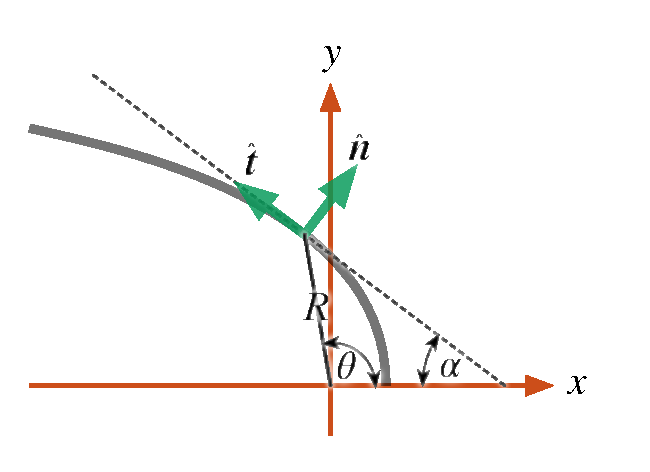
\includegraphics[width=0.6\linewidth]{./Figures/bowshock-unit-vectors}
  \caption{Vectores unitarios normal y tangente a la superficie $R(\theta)$
    en un plano de azimuth $\phi$ constante.}
    \label{fig:unit-vec}
\end{figure}


\subsection{Línea tangente}
\label{sec:tangent-line}
Debido a que el choque es ópticamente delgado y geométricamente
delgado, solo la región del choque cuya tangente sea paralela a la
línea de visión seré visible. Esto corresponde a una curva que
denominamos \textit{línea tangente}, que debe cumplir con la siguiente
condición:

\begin{align}
  \hat{n}'\boldsymbol{\cdot} \hat{z}' = 0
\end{align}

Denotamos como $\phi_T$ al ángulo azimutal que cumple la condición anterior
para una inclinación dada, en función del ángulo polar $\theta$:
\begin{align}
  \sin\phi_T = \tan i\tan\alpha = \tan i\frac{1+\omega\tan\theta}{\omega-\tan\theta}
  \label{eq:phi-tan}
\end{align}
De esta manera, la forma de la línea tangente del choque de proa, a la que llamamos
\textit{forma proyectada} viene dada por:

\begin{align}
  \left(
  \begin{array}{c}
    x'_T \\
    y'_T \\
    z'_T
  \end{array}
  \right) =
  R(\theta)\left(
  \begin{array}{c}
    \cos\theta\cos i - \sin\theta\sin\phi_t\sin i \\
    \sin\theta\left(1-\sin^2\phi_T\right)^{1/2} \\
    \cos\theta\sin i + \sin\theta\sin\phi_T\cos i
  \end{array}
  \right) \label{eq:proj-shape}
\end{align}
En el caso general, $z'_T$ no es una función lineal de $x'_T$ y $y'_T$, por lo que
la línea tangente no se encuentra en un plano.

La forma aparente $(x'_T, y'_T)$  de la línea tangente también puede escribirse
en coordenadas polares $(R', \theta')$, donde:
\begin{align}
  R'(\theta) = \left(x'^2_T + y'^2_T\right)^{1/2} & \mathrm{y} & \tan\theta' = \frac{y'_T}{x'_T}
  \label{eq:polar}
\end{align}
Es de notar a su vez que la ecuación (\ref{eq:phi-tan}) no tiene solución para valores
arbitrarios de $\theta$ y de la inclinación, puesto que se requiere que
$\left|\sin\phi_T\right| < 1$. Por tanto, la línea tangente solo existe para valores
de $\theta$ tales que $\theta < \theta_0$ donde $\theta_0$ es el valor de $\theta$ en
el eje de simetría de la línea tangente proyectada $(\theta'(\theta_0) = 0)$ y que se
obtiene de la siguiente ecuación implícita:
\begin{align}
  \tan\theta_0 = \frac{|\tan i| + \omega(\theta_0)}{1 - \omega(\theta_0)|\tan i|}
  \label{eq:th-0}
\end{align}
Esto implica que si el choque de proa es suficientemente ``abierto''
$(\alpha > \alpha_{min})$, entonces para inclinaciones tales que
$|i| > 90^\circ - \alpha_{min}$ no existirá la línea tangente para ningún valor de $\theta$,
es decir, el choque de proa se encontrará sufientemente ``de cara'' como para que ya no
parezca un choque de proa para el observador.

\subsection{Radios característicos en el plano del cielo}

En orden de comparar la forma $R(\theta)$ con observaciones, es útil definir los radios
característicos $R'_0$ y $R'_{90}$, donde $R'_0$ es el radio del eje de simetría aparente
y $R'_{90}$ es el radio aparente en la dirección perpendicular a $R'_0$. Es decir
$R'_0 = x'_T(y'_t=0)$ y $R'_{90} = y'_t(x'_t = 0)$. Utilizando las ecuaciones
(\ref{eq:phi-tan}) y (\ref{eq:proj-shape}) encontramos que:
\begin{align}
R'_0 = R(\theta_0)\cos(\theta_0 + i)
\label{eq:R0p}
\end{align}
Donde $\theta_0$ es la solución de la ecuación (\ref{eq:th-0}), y
\begin{align}
  R'_{90} = R(\theta_{90})\sin\theta_{90}\left(1-\sin^2\phi_T(\theta_{90})\right)^{1/2}
  \label{eq:R90p}
\end{align}
donde $\theta_{90}$ es la solución de la siguiente ecuación implícita:
\begin{align}
  \cot\theta_{90} = \frac{1 - \left(1+\omega(\theta_{90})^2\sin^22i\right)^{1/2}}
  {2\omega(\theta_{90})\cos^2i}
  \label{eq:th90}
\end{align}

\section{Cuádricas de Revolución}
\label{sec:quadrics}
\newcommand\Sin{\ensuremath{\mathcal{S}}}
\newcommand\Cos{\ensuremath{\mathcal{C}}}
\newcommand\Cot{\ensuremath{\mathcal{T}}}
\newcommand\Q{\ensuremath{\mathcal{Q}}}

En el caso general es difícil encontrar la forma aparente para un choque de
proa siguiendo el formalismo desarrollado en la sección anterior, por lo que
optamos por aproximar la forma éstos con una de las superficies más simples:
las \textit{cuádricas de revolución}, que son superficies de revolución de
las curvas cónicas. Dado el modelo general descrito en la \S \ref{sec:Modelo-generico}, haremos algunas restricciones para las superficies
cuádricas que utilizaremos en este trabajo:
\begin{itemize}
  \item El eje focal se encuentra alineado con el eje $x$
  \item La posición del foco de la superficie cuádrica no necesariamente coincide
    con la posición de la fuente
  \item En el caso de las hipérbolas, solo tomamos una de las ramas de ésta.
\end{itemize}
Implementando dichas restricciones, utilizamos la representación paramétrica de
las curvas cónicas en términos de un parámetro adimensional denotado con la letra
$t$:
\begin{align}
  x &= x_0 + \sigma a\Cos(t) \\
  y &= b\Sin(t) 
\end{align}
Donde:
\begin{align}
  \Cos(t), \Sin(t) &=\left\lbrace
  \begin{array}{lr}
    \cos{t}, \sin t & \mathrm{elipses}\\
    \cosh{t}, \sinh{t} & \mathrm{hipérbolas}       
  \end{array}\right. \\
  \sigma &= \left\lbrace
  \begin{array}{lr}
    +1 & \mathrm{elipses} \\
    -1 & \mathrm{hipérbolas}
  \end{array}\right. \\
  x_0 &= R_0 -\sigma a \label{eq:x0} 
\end{align}
Donde $a$ y $b$ representan la longitud de los semi-ejes de la cónica en cuestión (Figura \ref{fig:conics}).
$x_0$ representa la distancia entre el centro de la cónica y el origen. 

La forma polar del choque de proa $R(\theta)$ viene dada por:

\begin{align}
  \tan\theta &= \frac{b\Sin(t)}{a\Cos(t) + x_0} \label{eq:t-th-conversion} \\
  R &= \left(\left(a\Cos(t) + x_0\right)^2 + b^2\Sin^2(t)\right)^{1/2} 
\end{align}

El tipo de cónica lo podemos caracterizar mediante el parámetro $\Q$, donde:

\begin{align}
  \Q \equiv \sigma\frac{b^2}{a^2}
\end{align}

Para las superficies abiertas (hiperboloides) tenemos que $\Q < 0$, mientras que para las superficies cerradas tenemos que $\Q > 0$. Casos particulares son la esfera $\Q =1$ y el paraboloide $\Q = 0$. De manera equivalente se puede definir el ángulo $\theta_Q$ como sigue:

\begin{align}
  \tan\theta_Q = \sigma \frac{b}{a} \label{eq:thc}
\end{align}

Este ángulo se relaciona con la excentricidad de las cónicas (y que sustituye a esta última en este trabajo) como se muestra a continuación:

\begin{align}
  \tan\theta_Q = \sigma\sqrt{\left|1-e^2\right|}
\end{align}


\begin{figure}
  \begin{tabular}{cc}
    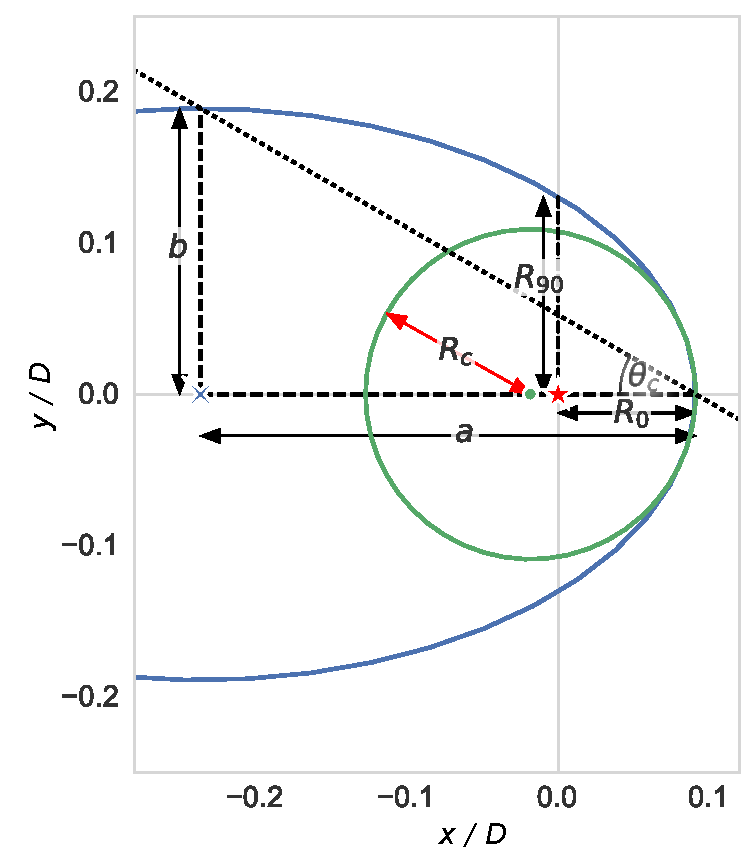
\includegraphics[width=0.4\linewidth]{./Figures/ellipse_edited} &
    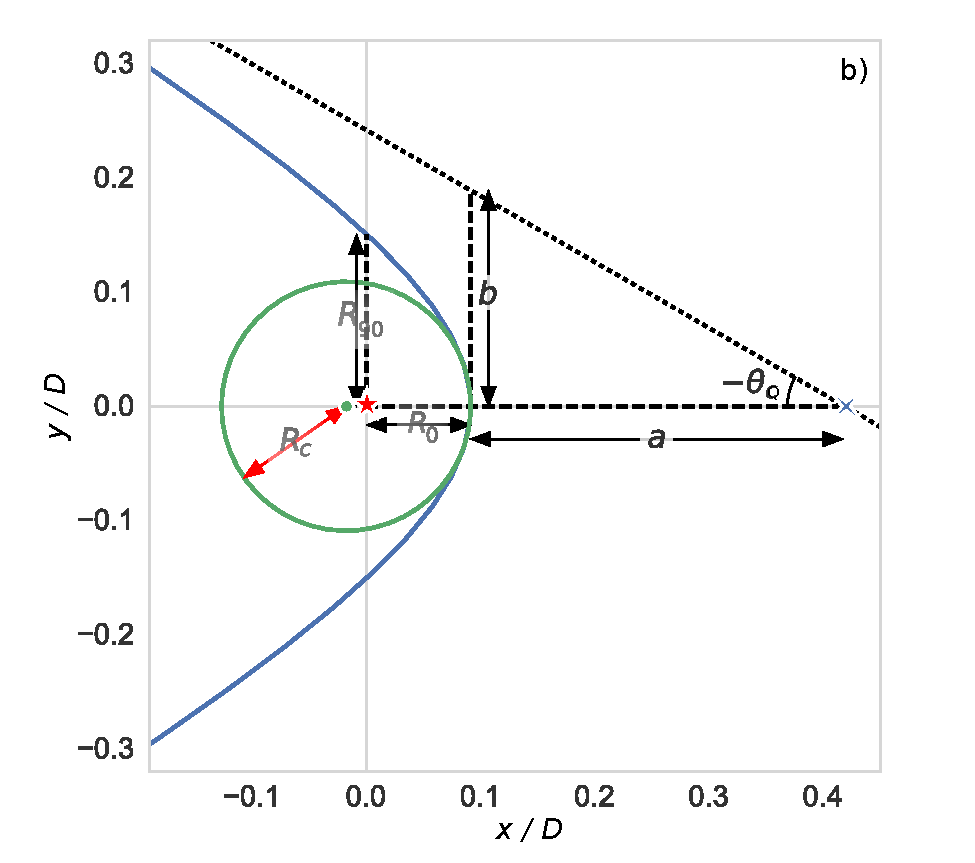
\includegraphics[width=0.5\linewidth]{./Figures/hyperbola_edited}
  \end{tabular}
  \caption{Representación esquemática de: Izquierda: Elipse. Y, derecha: Hipérbola. En ambos casos se ilustran los parámetros relevantes de éstas y los radios característicos}
  \label{fig:conics}
\end{figure}

\begin{figure}
  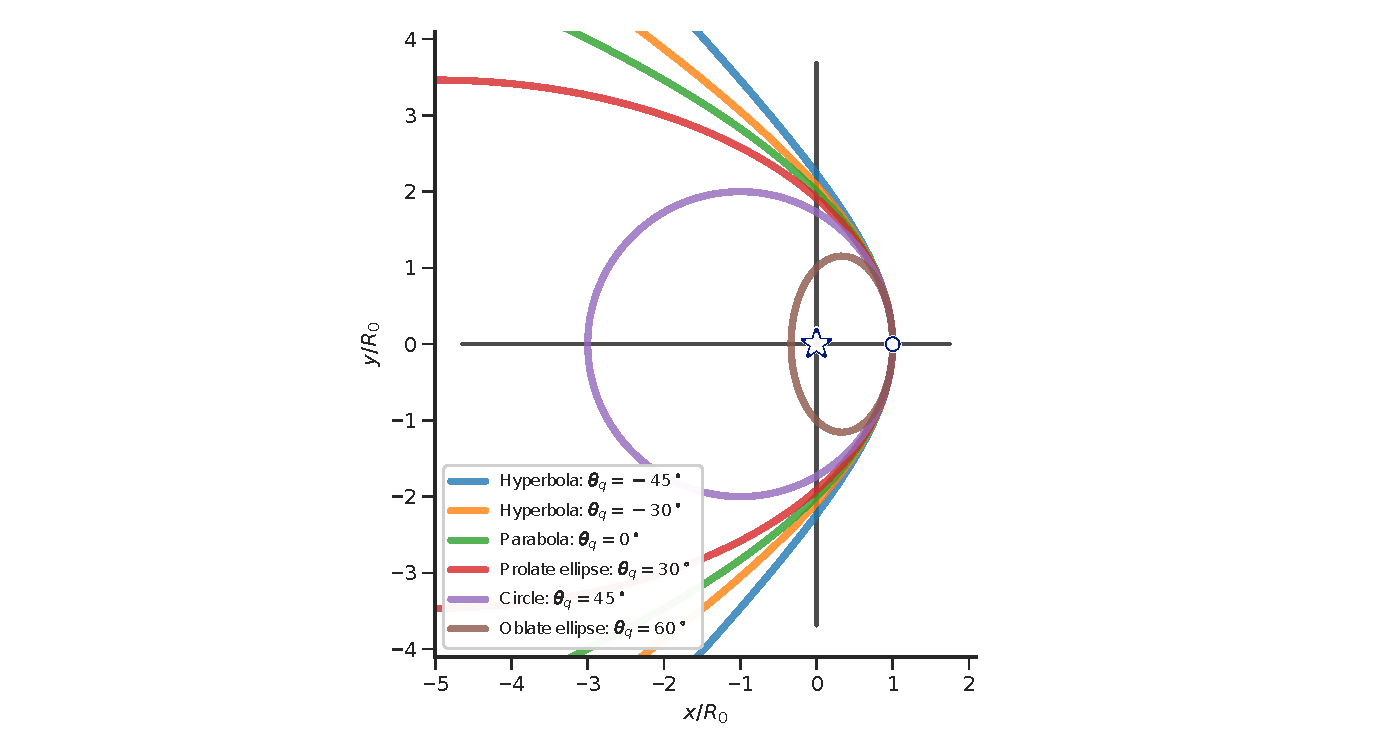
\includegraphics[width = 0.5\linewidth]{./Figures/conic1}
  \caption{Familia de curvas cónicas, donde el valor del parámetro $\theta_Q$ varía desde $\theta_Q < 0$ (hipérbolas) hasta $\theta_c > 0$ (elipses). Casos especiales son $\theta_Q = 0$ (parábola) y $\theta_Q = 45^\circ$ (círculo). Este parámetro sustituye en este trabajo a la excentricidad.}
  \label{fig:conics-family}
\end{figure}

%\subsection{Radios Característicos}
%\label{sec:conic-char-radii}
El set de parámetros $(a, x_0, \Q)$ es suficiente para caracterizar a nuestras cuádricas de revolución: $\Q$ nos indica el tipo de cónica, $a$ establece la escala y $x_0$ el desplazamiento del centro a lo largo del eje x. Sin embargo, para futuras aplicaciones tanto a modelos de interacción de vientos como a observaciones (capítulos \ref{chap:hipersonica} y \ref{chap:proplyds}) nos sería util hacer la caracterización mediante los parámetros $(R_0, \Pi, \Lambda)$ (ver \S \ref{sec:char-rad}). Las equivalencias entre los dos sets de parámetros los calculamos a continuación:

%Para que las curvas cónicas den una buena aproximación a la forma de un choque de proa dado, necesitamos saber calcular los radios característicos para éstas. A partir de la descripción de éstos en la \S \ref{sec:char-rad} podemos encontrar expresiones para cada uno de éstos en términos de los parámetros de las cónicas:

\begin{align}
  R_c &= \frac{b^2}{a} = a|\Q|\label{eq:R-curv-conic}\\
  R^2_{90} &= b^2\sigma\left(1 - \frac{x^2_0}{a^2}\right) = \Q\left(a^2 - x^2_0\right)\label{eq:R90-conic}
\end{align}

Combinando las ecuaciones (\ref{eq:x0})
%$R_0$ es independiente de los parámetros de las cónicas, por tanto, en esta sección nos será útil normalizar con este radio. De esta forma, podemos invertir las siguientes ecuaciones:

\begin{align}
  \tilde{a} &= \pm\frac{\tilde{R}_c}{2\tilde{R}_c - \tilde{R}_{90}^2} \label{eq:til-a}\\
  \tilde{b} &= \frac{\tilde{R}_c}{\left|2\tilde{R}_c - \tilde{R}_{90}^2\right|^{1/2}}\label{eq:til-b}\\
  \tan\theta_c &= \pm\left|2\tilde{R}_c - \tilde{R}_{90}^2\right|^{1/2} \label{eq:thc2}
\end{align}
Nótese que la cantidad $T_c\equiv 2\tilde{R}_c - \tilde{R}_{90}^2$ nos sirve como discriminante para distinguir el tipo de curva cónica que mejor ajusta a un choque de proa dado.

\subsection{Proyección en el plano del cielo}

El objetivo de esta sección es obtener la forma proyectada de las cuádricas de revolución, puesto que son una aproximación buena y mucho más sencilla a la forma real de un choque de proa. La forma tridimensional de las cuádricas de revolución viene dada por:

\begin{align}
  x &= a\Cos(t) + x_0 \\
  y &= b\Sin(t)\cos\phi \\
  z &= b\Sin(t)\sin\phi
\end{align}

Siguiendo el procedimiento mostrado en la \S \ref{sec:projection} calculamos el ángulo azimutal $\phi$ que cumple con el criterio de ser tangente al la línea de visión:

\begin{align}
  \sin\phi_T = \frac{b}{a}\tan i\Cot(t) 
\end{align}
Donde:
\begin{align}
  \Cot(t) = \left\lbrace
  \begin{array}{lr}
    \cot t & \mathrm{si}~\theta_c > 0 \\
    \coth t & \mathrm{si}~\theta_c < 0 
  \end{array}
  \right.
\end{align}

Ahora utilizamos la ecuación (\ref{eq:rotation}) para obtener la forma aparente de una cuádrica dada:

\begin{align}
  x'_T &= \frac{\Cos(t)}{a\cos i}\left(a^2\cos^2 i \pm b^2\sin^2 i\right) + x_0\cos i
  \label{eq:x-prime-proj}\\
  y'_T &= b\Sin(t)\left(1 - \frac{b^2}{a^2}\tan^2 i\Cot^2(t)\right)^{1/2}
  \label{eq:y-prime-proj}
\end{align}

Se espera que la forma proyectada de una cuádrica dada sea otra cuádrica del mismo tipo, por lo que es posible escribir las ecuaciones (\ref{eq:x-prime-proj}) y (\ref{eq:y-prime-proj}) de la siguiente manera: 

\begin{align}
  x'_T &= a'\Cos(t') + x'_0 \label{eq:xtprime}\\
  y'_T &= b'\Sin(t') \label{eq:ytprime}
\end{align}
Donde:
\begin{align}
  x'_0 &= x_0\cos i \\
  a' &= \left(a^2\cos^2 i \pm \b^2\sin^2 i\right)^{1/2} \label{eq:a-prime}\\
  b' &= b \label{eq:b-prime}\\
  \Cos(t') &= \frac{a'\Cos(t)}{a\cos i} \\
  \Sin(t') &= \left(1 - \Cos^2(t')\right)^{1/2}
\end{align}

Dos cantidades que nos van a ser de utilidad son los valores del parámetro $t$
que denominaremos $t_0$ y $t_{90}$ y son tales que $t'(t_0) = 0$ y $t'(t_{90}) = \frac{\pi}{2}$
o bien $y'_T(t_0) = 0$ y $x'_T(t_{90}) = 0$. De esta manera obtenemos las siguientes ecuaciones
implícitas evaluando las ecuaciones (\ref{eq:x-prime-proj}) y(\ref{eq:y-prime-proj}) en $t=t_{90}$
y $t=t_0$ respectivamente:

\begin{align}
  \Cot(t_0) &= \frac{a}{b}\cot{i} = \frac{\cot{i}}{\left|\tan\theta_c\right|} \label{eq:t0}\\
  \Cos(t_{90}) &= -\frac{ax_0\cos^2{i}}{a^2\cos^2{i}\pm b^2\sin^2{i}} \label{eq:t90}
\end{align}

Los radios característicos aparentes los podemos calcular a partir de las ecuaciones (\ref{eq:xtprime}) y
(\ref{eq:ytprime}) como se hizo para los radios característicos en el sistema no primado:

\begin{align}
  R'_0 &= \pm a' + x'_0\\
  R'_c &= \frac{b'^2}{a'}\\
  \tan\theta'_c &= \pm\frac{b'}{a'} \\
  R'_{90} &= \left(2R'_c \mp \tan^2\theta'_c\right)^{1/2}
\end{align}

Utilizando las ecuaciones (\ref{eq:x0}), (\ref{eq:a-prime}) y (\ref{eq:b-prime}),
utlizando la definición $D' = D\cos i$ e introduciendo la función
$f(i;\theta_c)\equiv \left(1 \pm \tan^2\theta_c\tan^2i\right)^{1/2}$ obtenemos
ecuaciones explícitas para los radios característicos en el sistema de referencia
del plano del cielo en términos de la inclinación:

\begin{align}
  \frac{q'}{q} &= 1 \pm \tilde{R}_c\cot^2\theta_c\left(f(i;\theta_c) - 1\right) \\
  \tilde{R}'_c &= \frac{\tilde{R_c}}{\cos^2if(i;\theta_c)\frac{q'}{q}} \label{eq:Rpc-quad}\\
  \tan\theta'_c &= \frac{\tan\theta_c}{\cos if(i;\theta_c)} \label{eq:thcp-quad}\\
  \tilde{R}'_{90} &= \left(\frac{2\tilde{R}_cf(i;\theta_c) \mp
                    \tan^2\theta_c\frac{q'}{q}}{q'/q}\right)^{1/2}\frac{\sec i}{f(i;\theta_c)}
                    \label{eq:Rp90-quad}
\end{align}

Cuando $\tilde{R}'_{90}$ es medible, entonces es posible hacer diagramas de diagnóstico como
el de la figura \ref{fig:diagnostic} para comparar con observaciones, independientemente de cualquier modelo de choques de proa.

\begin{figure}
  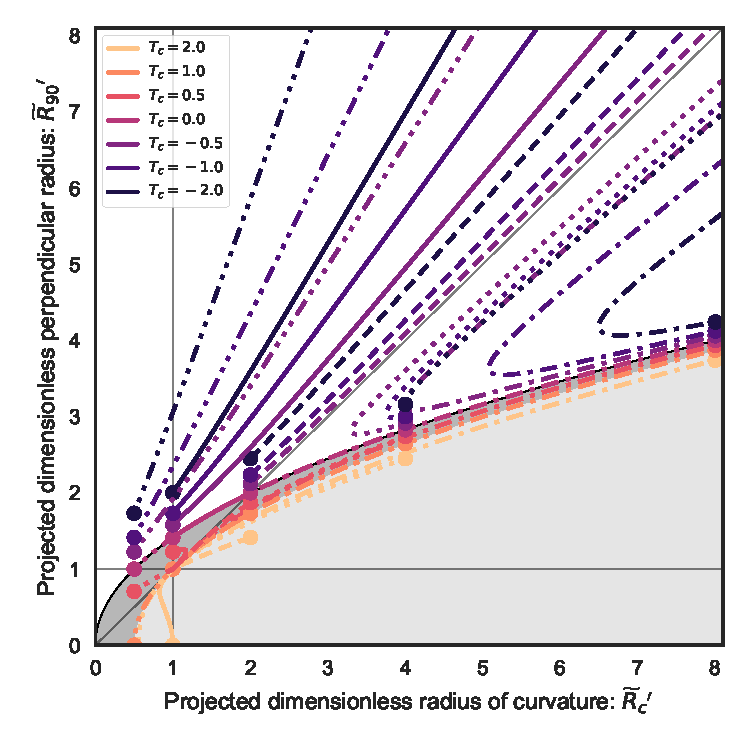
\includegraphics[width=0.5\linewidth]{./Figures/projected-R90-vs-Rc}
  \caption{Diagrama de diagnóstico $\tilde{R}'_{90}$ vs $\tilde{R}'_c$ para las cuádricas de revolución. En la región sin sombrear se representan las superficies abiertas (hiperboloides, $\theta_c <0$), mientras que la región más oscura representa a elipsoides prolatos  $(0 < \theta_c < 45^\circ)$ y la región poco sombreada a elipsoides oblatos $(\theta_c > 45^\circ)$}
  \label{fig:diagnostic}
\end{figure}

%Buscamos adjuntar el paper ``quadrics bowshock''

\chapter{Herramientas de Programación}
\label{chap:hipersonica}

El problema de interacción de dos vientos es de gran interés en astrofísica, y
ha sido estudiado en múltiples ocasiones, principalmente mediante simulaciones
hidrodinámicas. Sin embargo, cuando se toman en cuenta diversos factores, incluídos
conservación de masa, momento y momento angular, el problema puede resolverse de manera
algebraica.
\section[Conservación]{Cantidades conservadas en un flujo hipersónico de capa delgada}

Consideramos dos flujos hipersónicos, no acelerados que forman una capa estacionaria delgada
formada por dos choques radiativos separados por una discontinuidad de contacto. El sistema
tiene geometría cilíndrica y los vientos no tienen velocidad azimutal. Bajo estos términos,
describimos la posición de la capa delgada como $R(\theta)$, donde $R$ es el radio de la capa
medido a partir de la posición del origen del viento con menor momento y $\theta$ es el ángulo
polar. Si asumimos que el gas chocado está bien mezclado, entonces tiene una sola velocidad
pos choque dada por:

\begin{align}
  \vec{v} = v_r \hat{r} + v_z \hat{z}
\end{align}

Donde el eje de simetría del sistema es paralelo a $\hat{z}$, y $\hat{r}$ es el radio cilíndrico.
Definimos $\dot{M}(\theta)$, $\vec{\dot{\Pi}}(\theta)$ y $\dot{J}(\theta)$ como la tasa de pérdida
de masa, la tasa de momento y la tasa de momento angular, respectivamente, de la capa delgada
integradas desde $\theta=0$ hasta $\theta$. Éstas se calculan de la siguiente manera:

\begin{align}
  \vec{\dot{\Pi}}(\theta) &= \dot{\Pi}_r(\theta) \hat{r} + \dot{\Pi}_z(\theta) \hat{z} = \dot{M}\left(
                      v_r \hat{r} + v_z\hat{z}\right) \label{eq:dot-pi}\\
  \vec{\dot{J}}(\theta) &= \vec{R}(\theta) \times \vec{\dot{\Pi}}(\theta)  \\
  \dot{M}(\theta) &= \dot{M}_w(\theta) + \dot{M}_{w1} \label{eq:dot-M}
\end{align}
Donde $\vec{R}(\theta)\equiv R(\theta)\sin\theta~\hat{r} + R(\theta)\cos\theta~\hat{z}$. Resolviendo el producto
cruz y tomando su magnitud encontramos que:

\begin{align}
  \dot{J}(\theta) &= \dot{M}(\theta)R(\theta)v_\theta \label{eq:dot-J}\\
  \mathrm{donde:~} & v_\theta = v_r\cos\theta - v_z\sin\theta \label{eq:v-theta}
\end{align}

Por otro lado, al asumir estado estacionario, necesitamos que la tasa de pérdida de masa, la tasa de
momento y la tasa de momento angular de la capa delgada sean iguales a aquellas inyectadas por los dos
vientos. Entonces definimos estas cantidades como $\dot{M}_w$, $\dot{\Pi}_{wr}$, $\dot{\Pi}_{wz}$ y
$\dot{J}_{w}$ para el viento con menor momento, y para el otro viento se utiliza la misma notación
solo que utilizando el subíndice ``w1''. De esta forma tenemos que:
\begin{align}
  \dot{\Pi}_r(\theta)\hat{r} + \dot{\Pi}_z(\theta)\hat{z} &= \left[\dot{\Pi}_{wr}(\theta)+ \dot{\Pi}_{wr1}(\theta)
                                                            \right]\hat{r} + \left[\dot{\Pi}_{wz}(\theta)+ \dot{\Pi}_{wz1}(\theta)\right]\hat{z}
                                                            \label{eq:Pi-2} \\
  \dot{J} &=\dot{J}_w(\theta) + \dot{J}_{w1}(\theta) \label{eq:J-2}\\
  \dot{M}(\theta) &= \dot{M}_w(\theta) + \dot{M}_{w1}(\theta) \label{eq:M-2}
\end{align}

Combinando las ecuaciones (\ref{eq:dot-pi}), (\ref{eq:dot-J}), (\ref{eq:dot-M}), (\ref{eq:Pi-2}), (\ref{eq:J-2}) y (\ref{eq:M-2})
encontramos que:

\begin{align}
  \dot{M}(\theta)\left[v_r \hat{r} + v_z\hat{z}\right] &= \left(\dot{\Pi}_{wr}(\theta) + \dot{\Pi}_{wr1}(\theta)\right)\hat{r} +
                                                         \left(\dot{\Pi}_{wz}(\theta) + \dot{\Pi}_{wz1}(\theta)\right)\hat{z} \\
  \dot{M}(\theta)v_\theta R(\theta) &= \dot{J}_w(\theta) + \dot(J)_{w1}(\theta)
\end{align}
Y finalmente combinando con la ecuación (\ref{eq:v-theta}) resolvemos para $R(\theta)$:
\begin{align}
  R(\theta) = \frac{\dot{J}_w(\theta) + \dot(J)_{w1}(\theta)}{\left(\dot{\Pi}_{wr}(\theta) + \dot{\Pi}_{wr1}(\theta)\right)\cos\theta
  - \left(\dot{\Pi}_{wz}(\theta) + \dot{\Pi}_{wz1}(\theta)\right)\sin\theta} \label{eq:R-wind}
\end{align}



\section[Dos Vientos]{Problema de Interacción de Dos Vientos}
\label{sec:CRW-2-winds}
Aplicamos el formalismo ya mencionado para la interacción de dos vientos radiales. El viento con menor momento
se localiza en el origen, y su densidad a radio fijo varía con el ángulo polar como una ley de potencias
(figura \ref{fig:isotropic-aniso}):
\begin{align}
  n(\theta) = n_0\cos^k\theta \label{eq:anisotropic-density}
\end{align}
Donde el índice $k$ indica el grado de anisotropía del viento ``interno''. Algunos casos particularmente interesantes
son el viento para un proplyd \citep{HA:1998}, donde $(k=1/2)$ y el caso ``isotrópico'' \citep{Canto:1996} donde $k=0$.
Por el momento restringimos al viento ``externo'' como isotrópico. El problema se muestra de manera esquemática en la
figura \ref{fig:crw-esquema}.

Utilizando la ecuación (\ref{eq:anisotropic-density}) encontramos que la tasa de pérdida de masa está dada por:

\begin{align}
  \dot{M}_w = \int^\theta_0\int^{2\pi}_0\rho_w v_w~d\theta~d\phi =
  \frac{M^0_w}{2\left(k+1\right)}\left(1 - \cos^{k+1}\theta\right) \label{eq:inner-dot-M}
\end{align}
Donde $v_w$ es la velocidad del viento inteno, $\rho_w = n\bar{m}$  es su densidad, $n$ se obtiene de la ecuación
(\ref{eq:anisotropic-density}), $M^0_w = 4\pi r^2_0v_w n_0 \bar{m}$ es la tasa de pérdida de masa integrada hasta
$\theta = \pi$ para el caso isotrópico, $\bar{m}$  es la masa promedio de las partículas del viento y
$r_0$ es el radio del viento al cual se alcanza la velocidad terminal $v_w$. Para un proplyd consideramos que dicho
radio es el del frente de ionización.

Con esto, obtenemos las tasas de momento y momento angular:
\begin{align}
  \dot{\Pi}_{wz} &= \int^\theta_0 v_w\cos\theta~d\dot{M}_w =
                   \frac{v_w \dot{M}^0_w}{2\left(k+2\right)}\left(1 - \cos^{k+2}\theta\right) \label{eq:Pi-wz} \\
  \dot{\Pi}_{wr} &= \int^\theta_0 v_w\sin\theta~d\dot{M}_w = \frac{1}{2}\dot{M}^0_w v_w I_k(\theta) \\
  \dot{J}_w &= \int^\theta_0 |\vec{R} \times \vec{v}_w|d\dot{M}_w = 0 \label{eq:inner-dot-J}
\end{align}

Donde la integral $I_k(\theta) = \int^\theta_0 \cos^k\theta \sin^2\theta~d\theta$ tiene solución analítica para $k=0$,
es una integral elíptica de segundo tipo cuando $k=\frac{1}{2}$ y su solución es aun más compleja para el resto de los
casos. Las tasa de momento angular para el viento interior es cero debido a que éste se mide respecto al origen, donde
se localiza la fuente con menor momento. En este punto los vectores de posición y velocidad para un valor de $\theta$
dado son paralelos.

Para el viento exterior consideramos dos casos principales: un viento esférico e isotrópico y un viento
plano--paralelo de densidad y velocidad constante.

\subsection{Interacción con un viento esférico isotrópico}
\label{sec:mod-isotropic}
En este caso tomamos como variable independiente al ángulo polar medido a partir de la posición de la fuente del viento
externo, denotado por $\theta_1$. De esta forma las tasas de pérdida de masa, momento y momento angular quedan como sigue:

\begin{align}
  \dot{M}_{w1} &= \frac{M^0_{w1}}{2}\left(1 - \cos\theta_1\right)\\
  \dot{\Pi}_{wz1} &= -\frac{v_{w1}\dot{M}^0_{w1}}{4}\sin^2\theta_1\\
  \dot{\Pi}_{wr1} &= \frac{v_{w1}\dot{M}^0_{w1}}{4}\left(\theta_1 - \sin\theta_1\cos\theta_1\right)\\
  \dot{J}_{w1} &= \int^{\theta_1}_0 R(\theta)v_{w1}\sin(\pi-\theta-\theta_1)~d\dot{M}_{w1} \label{eq:J1}
\end{align}

Utilizando la ley de los senos (ver figura \ref{fig:crw-esquema}), la ecuación (\ref{eq:J1}) queda como sigue:

\begin{align}
  \dot{J}_{w1} &= Dv_{w1}\int^{\theta_1}_0 \sin\theta_1~d\dot{M}_{w1} =
                 \frac{v_{w1}\dot{M}^0_{w1}}{4}\left(\theta_1 - \sin\theta_1\cos\theta_1\right) D \label{eq:J1-iso}
\end{align}

Por otro lado, de la figura \ref{fig:crw-esquema}, podemos deducir la siguiente relación geométrica entre $R(\theta)$,
$\theta$ y $\theta_1$:
\begin{align}
  \frac{R(\theta)}{D} &= \frac{\sin\theta_1}{\sin(\theta+\theta_1)} \label{eq:R-geometric}
\end{align}

Combinando las ecuaciones (\ref{eq:R-wind}), (\ref{eq:Pi-wz}) - (\ref{eq:J1-iso}) y (\ref{eq:R-geometric}) obtenemos una ecuación
implícita que nos indica la dependencia de $\theta_1$ con $\theta$:

\begin{align}
  \theta_1\cot\theta_1 -1 = 2\beta I_k(\theta)\cot\theta - \frac{2\beta}{k+2}\left(1 - \cos^{k+2}\theta\right) \label{eq:th1-th} 
\end{align}
Donde $\beta = \frac{\dot{M}^0_w v_w}{\dot{M}^0_{w1}v_{w1}}$ es el cociente del momentos entre los vientos. Este parámetro, junto con el
índice de anisotropía $k$ son los que determinan la forma del choque de proa. 

Los radios característicos en este caso se muestran a continuación. El procedimiento detallado se puede consultar en el apéndice
\ref{app:derivation-radii}:

\begin{align}
  \frac{R_0}{D} &= \frac{\beta^{1/2}}{1+\beta^{1/2}} \\
    \tilde{R}_{90} &= \frac{\left(3\xi\right)^{1/2}\left(1+\beta^{1/2}\right)}
                     {\left(1+\frac{1}{5}\xi\beta\right)^{1/2}\left(1-\xi\beta\right)} \label{eq:CRW-R90}\\
  \tilde{R}_c &= \left|1 - 2\gamma\right|^{-1} \label{eq:CRW-Rc}\\
  \mathrm{Donde:~} \gamma &= \frac{C_{k\beta}}{1+\beta^{1/2}} + \frac{1 + 2\beta^{1/2}}{6} 
\end{align}


\subsection{Interacción de un viento esférico isotrópico con un viento plano--paralelo}

En este caso las tasas de pérdida de masa, de momento y momento angular del viento plano--paralelo con velocidad $v_a$ y
densidad uniforme $\rho_a$ quedan como sigue:

\begin{align}
  \dot{M}_{w1} &= \pi \rho_a v_a R^2 \sin^2\theta\\
  \dot{\Pi}_{wz1} &= - \pi\rho_a v^2_a R^2 \sin^2\theta\\
  \dot{\Pi}_{wr1} &= 0 \\
  \dot{J}_{w1} &= \int^r_0 r'v_a \sin\theta~d\dot{M}_{w1} = \frac{2}{3}\pi\rho_a v_a^2 R^3 \sin^3\theta 
\end{align}

Sustituyendo estas ecuaciones en (\ref{eq:R-wind}) junto con (\ref{eq:inner-dot-M}) - (\ref{eq:inner-dot-J})
para el caso isotrópico $(k=0)$ obtenemos lo siguiente:

\begin{align}
  R = \frac{\frac{2}{3}\pi\rho_a v_a R^3 \sin^3\theta}{\frac{\dot{M}^0_w v_w}{4}\left(\theta-\sin\theta\cos\theta\right)\cos\theta
  - \left(\frac{\dot{M}^0_w v_w}{4}\sin^2\theta - \pi\rho_a v^2_a R^2 \sin^2\theta\right)\sin\theta}
\end{align}

La condición de equilibrio de presión en este caso nos lleva a la siguiente relación:

\begin{align}
  \frac{\dot{M}^0_w v_w}{4\pi R^2_0} = \rho_a v^2_a \label{eq:Wilkin-stagnation}
\end{align}

Por tanto:

\begin{align}
  \tilde{R} = \frac{\frac{2}{3}\tilde{R}^3 \sin^3\theta}{\left(\theta-\sin\theta\cos\theta\right)\cos\theta
  - \left(\sin^2\theta - \tilde{R}^2 \sin^2\theta\right)\sin\theta}
\end{align}

Resolviendo para $\tilde{R}$ encontramos que:

\begin{align}
  \tilde{R} = \left[\csc^2\theta\left(1 - \theta\cot\theta\right)\right]^{1/2} \label{eq:R-Wilkin}
\end{align}

\subsection{Radios Característicos}
\label{sec:Wilkin-Char-Radii}

En este caso los radios característicos se calculan de la siguiente manera:

$R_0$ se obtiene directamente de la ecuación (\ref{eq:Wilkin-stagnation}) como
\begin{align}
  R_0 = \left(\frac{\dot{M}^0_w v_w}{4\pi \rho_a v^2_a}\right)^{1/2}
\end{align}

$R_{90}$ se calcula evaluando la ecuación (\ref{eq:R-Wilkin}) en $\theta=\frac{\pi}{2}$:

\begin{align}
  \tilde{R}_{90} = \sqrt{3} \label{eq:R90-Wilkin}
\end{align}

Por último, el radio de curvatura se obtiene haciendo una expansión de la ecuación (\ref{eq:R-Wilkin}) y
encontrando el coeficiente de segundo órden. El procedimiento detallado se muestra en el apéndice \ref{sec:Rc-Wilkin}:

\begin{align}
\tilde{R}_c = \frac{5}{3} \label{eq:Rc-Wilkin}
\end{align}

\chapter{The Work}
\chapter{Obtención de la Forma Aparente de los Choques en el Modelo de Aproximación Hipersónica}
La obtención de la forma aparente de los Radios Característicos de los choques de Proa
no se obtiene de manera analítica de forma sencilla, por lo que recurrimos a hacer
aproximaciones a la forma de un choque dado, utilizando las cuádricas de revolución.
Éstas cuádricas dan un buen ajuste pero no son capaces de reproducir la forma completa
de un choque de proa dado, por lo que recurrimos al uso de dos cuádricas que en conjunto
ajustan a la forma completa del choque: una para la ``cabeza'' del choque, y otro para la cola.
Y cómo ya vimos en la sección , los radios característicos aparentes se pueden obtener de
manera sencilla para estas superficies.

\begin{figure*}
  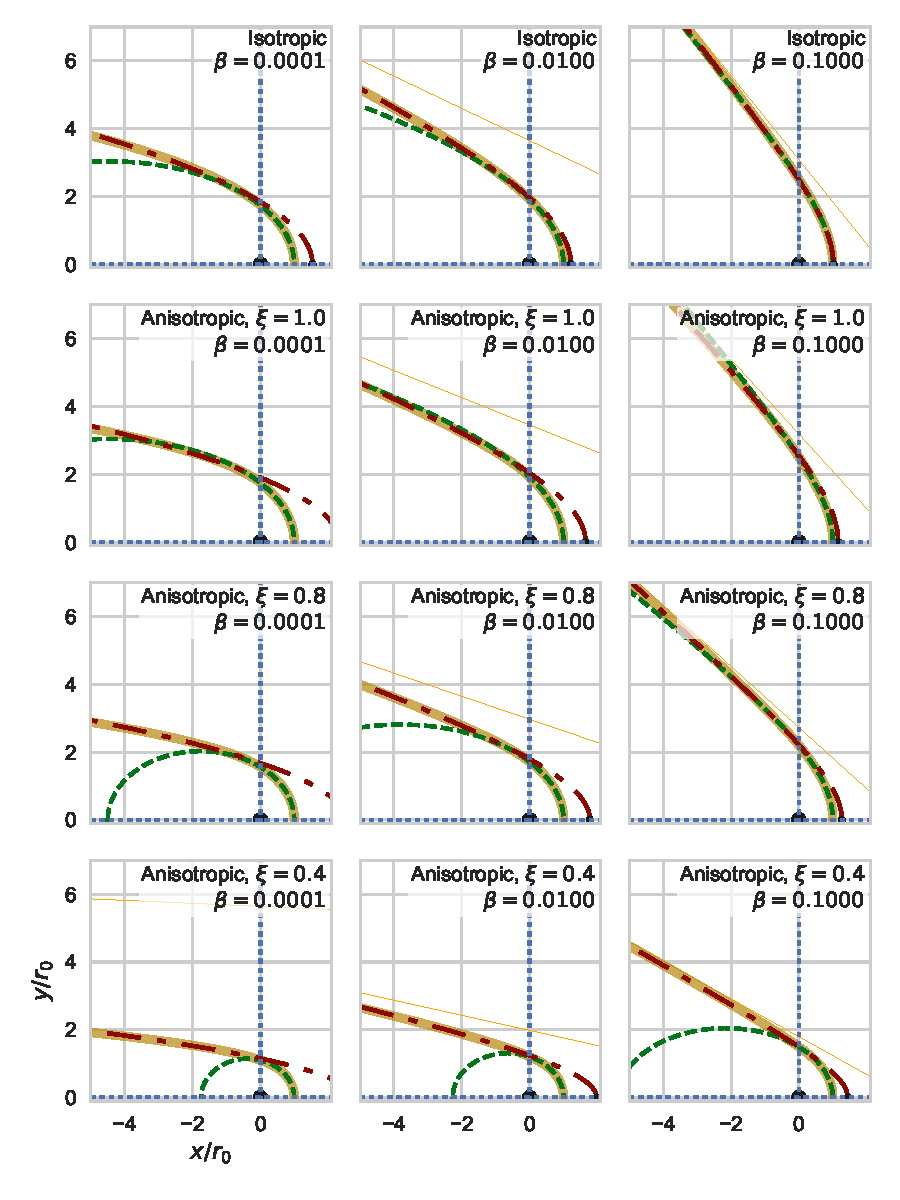
\includegraphics[width = 0.8\linewidth]{./Figures/conic-head-tail-analytic}
  \label{fig:conic-head-tail-fit}
  \caption{Ajuste de dos cuádricas a las soluciones de capa delgada. La línea gruesa continua
    representa la forma de un choque bajo la aproximación de capa delgada (capítulo
    \ref{chap:hipersonica}) para los parámetros enlistados en cada pánel. La línea verde es el
    ajuste obtenido para la cabeza, mientras que la roja corresponde al ajuste para la cola.}
\end{figure*}


\section{Ajustes a la cabeza}

Utilizando las ecuación (\ref{eq:thc2})  de la \S \ref{sec:conic-char-radii} y las ecuaciones
(\ref{eq:CRW-Rc}) y (\ref{eq:CRW-R90}) de la \S \ref{sec:CRW-2-winds} podemos calcular el parámetro
$\theta_c$ que nos indicará el tipo de cónica que ajusta mejor a cada solución del modelo de capa delgada
en función de los parámetros $\beta$ y $\xi$: 

 \begin{align}
   \tan\theta_c = \pm\left|\frac{3\xi\left(1 + \beta^{1/2}\right)^2}{\left(1 - \xi\beta\right)^2
   \left(1 + \frac{1}{5}\xi\beta\right)} - \frac{2}{\left|1 - 2\gamma\right|}\right|^{1/2}
 \end{align}

 En la figura  se ilustra la dependencia de $\theta_c$ con los parámetros $\beta$ y $\xi$, así como al tipo de
 cónica que ajusta mejor tanto la cabeza como la cola de cada solución a la forma de los choques de proa.
 
 \section{Ajustes a la cola}

 En el caso general del problema de capa delgada, el comportamiento de la cola tiende a ser hiperbólico, dado que
 el ángulo polar $\theta$ tiende a un valor asintótico denominado como $\theta_\infty$. Este ángulo es tal que
 $\theta_\infty + \theta_{1\infty} = \pi$ y se calcula resolviendo la siguiente ecuación explícita:

 \begin{align}
   
 \end{align}

 El ajuste a la hipérbola se logra ajustando tres parámetros fundamentales: $\theta_c = \theta_\infty - \pi$,
 la distancia entre la hipérbola y el centro de ésta a lo largo del eje focal $a_t$ y la distancia entre el origen
 y el centro de la hipérbola $x_{0,t}$. $a_t$ y $x_{0,t}$ se obtienen inicialmente con un ajuste numérico para una
 malla de valores de $\beta$ y $\xi$. Posteriormente hacemos tres ajustes anidados en tres niveles para determinar
 de manera analítica los parámetros de la hipérbola en función de $\beta$ y $\xi$. A continuación mostramos las
 funciones y los parámetros que mejor ajustan a la cola para cada solución a la forma de los choques de proa:

 \begin{align}
   x_{0,t} = 0.7\beta^{-0.55}\left[C_3\left(\log_{10}\beta\right)^3 + C_2\left(\log_{10}\beta\right)^2 +
   C_1\left(\log_{10}\beta\right) + C_0\right] \label{eq:tail-analytic-x0}\\
   (x_{0,t} - a_t) = D_2\left(\log_{10}\beta\right)^2 + D_1\left(\log_{10}\beta\right) + D_0
   \label{eq:tail-analytic-x0-minus-a}
 \end{align}

 Donde:
 
 \begin{alignat}{2}
   \label{eq:tail-analytic-coeffs-c}
   C_k &= c_{2,k}\xi^2 + c_{1,k}\xi + c_{0,k} & \mathrm{para~}k=[0,1,2,3] \\
   \label{eq:tail-analytic-coeffs-d}
   D_k &= d_{2,k}\xi^2 + d_{1,k}\xi + d_{0,k} & \mathrm{para~}k=[0,1,2]
 \end{alignat}

 Los coeficientes de los ajustes para la cola se muestran en la tabla \ref{tab:tail-fit-coeffs}:


\newcommand\iso{\ensuremath{^{\mathrm{iso}}}}

\begin{table}
  \caption{Coeficientes del ajuste hiperbólico a la cola de los choques de Proa}
  \label{tab:tail-fit-coeffs}
  \renewcommand\arraystretch{1.2}
  \setlength\tabcolsep{0.5\tabcolsep}
  \begin{tabular}{@{}llll@{}}
    \toprule
    Ecuación~(\ref{eq:tail-analytic-x0}) & 
    \multicolumn{3}{l}{
    Ecuación~(\ref{eq:tail-analytic-coeffs-c}) \dotfill
    } \\ \midrule
    \( C\iso_0 = +1.3195     \)    
    & \( c_{0,0} = +2.0758   \)  
    & \( c_{1,0} = -0.2309   \)  
    & \( c_{2,0} = -0.2532   \)\\
      \( C\iso_1 = +0.4229     \)    
    & \( c_{0,1} = +0.9571   \)  
    & \( c_{1,1} = -0.1530   \)  
    & \( c_{2,1} = -0.2487   \)\\
      \( C\iso_2 = +0.1092     \)    
    & \( c_{0,2} = +0.2528   \)  
    & \( c_{1,2} = -0.0360   \)  
    & \( c_{2,2} = -0.0794   \)\\
      \( C\iso_3 = +0.0051     \)    
    & \( c_{0,3} = +0.0171   \)  
    & \( c_{1,3} = -0.0010   \)  
    & \( c_{2,3} = -0.0095   \)\\ \midrule
    Ecuación~(\ref{eq:tail-analytic-x0-minus-a}) &
    \multicolumn{3}{l}{
    Ecuación~(\ref{eq:tail-analytic-coeffs-d}) \dotfill
    } \\ \midrule
    \( D\iso_0 = +0.7962   \)    
    & \( d_{0,0} = +0.8516 \)  
    & \( d_{1,0} = -0.0907 \)  
    & \( d_{2,0} = -0.2002 \)\\
      \( D\iso_1 = -0.2363   \)    
    & \( d_{0,1} = -0.7620 \)  
    & \( d_{1,1} = +0.1411 \)  
    & \( d_{2,1} = -0.0295 \)\\
      \( D\iso_2 = -0.0126   \)    
    & \( d_{0,2} = -0.0683 \)  
    & \( d_{1,2} = +0.0390 \)  
    & \( d_{2,2} = -0.0236 \)\\
    \bottomrule
  \end{tabular}
\end{table}

 
 En el apéndice  se muestran los detalles de cómo se obtuvieron los coeficientes de la tabla \ref{tab:tail-fit-coeffs}.
 
 \subsection{Ajustes a la cabeza y la cola en el caso de la interacción con un viento plano--paralelo}

 En este caso el ajuste a la cabeza es muy simple, utilizando los resultados para sus radios característicos
 (ecuaciones (\ref{eq:R90-Wilkin}) y (\ref{eq:Rc-Wilkin})) encontramos que el ajuste a la cabeza corresponde
 con una elipse tal que $\tan\theta_c = \frac{1}{3}$.

 Para el ajuste a la cola encontramos que ninguna de las cuádricas da una buena aproximación a la forma de la
 cola, pero contamos con la forma explícita del choque de proa (ecuación (\ref{eq:R-Wilkin})) así que ningún
 ajuste fue necesario.
 
 \section{Proyección en el plano del cielo para el modelo de capa delgada}

 La proyección en el plano del cielo se realizó utilizando las ecuaciones (\ref{eq:Rpc-quad}), (\ref{eq:thcp-quad})
 y (\ref{eq:Rp90-quad}) para los ajuste de la cabeza y de la cola, respectivamente.

 En la figura \ref{fig:residuals} se muestra el residuo del ajuste de diferentes soluciones contra el ángulo polar
 $\theta$. Se puede apreciar que para cierto valor de $\theta$, que podemos denominar como $\theta_{tran}$, ocurre
 la transición donde el mejor ajuste deja de ser el de la cabeza y el ajuste de la cola empieza a ser más efectivo.
 Debido a esto, tenemos que tener cuidado qué ajuste elegir para calcular los radios característicos aparentes. Si
 $\theta_0 < \theta_{tran}$ entonces podemos utilizar el ajuste a la cabeza para calcular el radio de curvatura
 aparente, en caso contrario se tiene que utilizar el ajuste a la cola, lo que ocurre a inclinaciones altas.
 Para calcular $R'_{90}$ hay que vigilar si $\theta_{90}$ es mayor o menor a $\theta_{tran}$ para decidir qué ajuste
 utilizar. En este último caso será el de la cola para la mayoría de las inclinaciones.

 \begin{figure}
   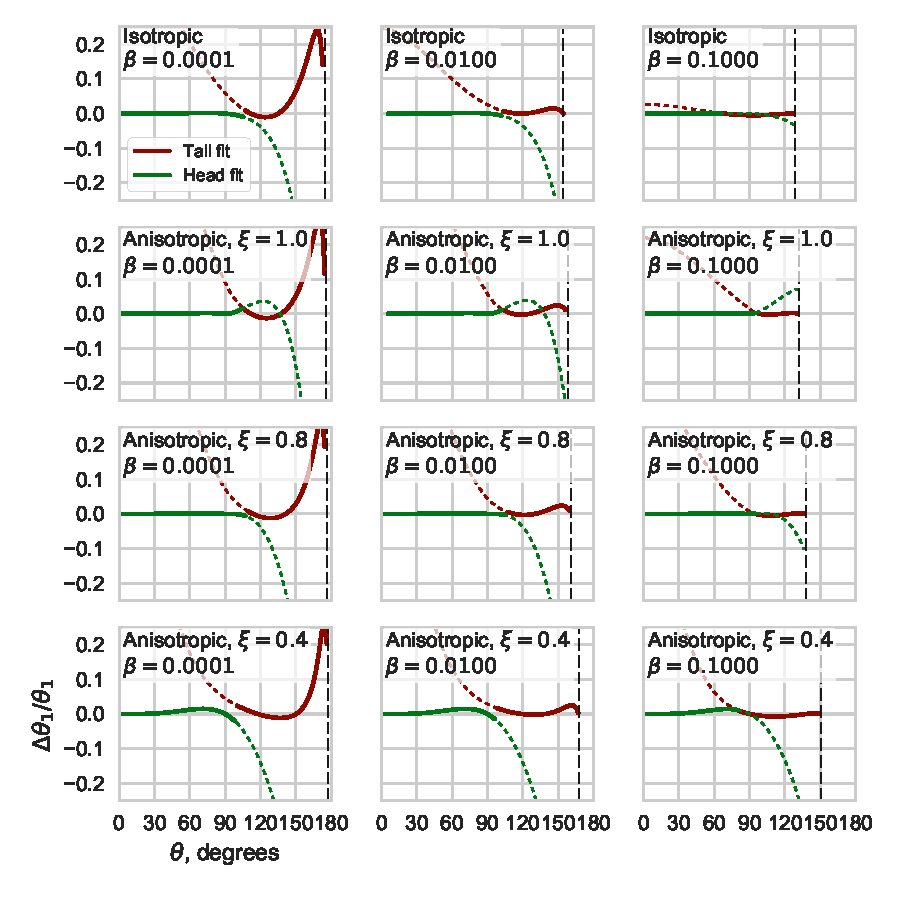
\includegraphics[width=0.5\linewidth]{./Figures/conic-head-tail-residuals}
   \caption{Residuo del ajuste de las cónicas a la forma del choque. La línea verde muestra el residuo del ajuste a la cabeza y la roja el ajuste a la cola. En todos los casos existe un valor de $\theta_{tran}$ donde para $\theta < \theta_{tran}$ el mejor ajuste es el de la cabeza y para $\theta \geq \theta_{tran}$ el mejor ajuste es el de la cola}.
   \label{fig:residuals}
 \end{figure}

 Utilizando las ecuaciones (\ref{eq:t-th-conversion}), (\ref{eq:t0}) y (\ref{eq:t90}) calculamos los valores para $\theta_0$
 y $\theta_{90}$ para las cuádricas:

 \begin{align}
   \cot\theta_0 = \cot\theta_c\cot{i} + \frac{x_0}{b} \sqrt{\cot^2\theta_c\cot^2{i}\pm 1}
 \end{align}

 Utilizando las ecuaciones (\ref{eq:x0}), (\ref{eq:til-b}) y (\ref{eq:thc2}) encontramos que:

 \begin{align}
   \frac{x_0}{b} = \frac{|\tan\theta_c|}{\tilde{R}_c} - |\cot\theta_c|
 \end{align}

 Por otro lado:

 \begin{align}
   \Cot(\theta_{90}) = f_2(i;\theta_c)\left[\frac{x_0}{b} - \frac{x_0}{a}\frac{|\cot \theta_c|}{f^2(i;\theta_c)}\right] 
 \end{align}

 Donde $f(i;\theta_c)$ fue definido en la sección \ref{sec:quadrics} y:
 \begin{align}
   f_2(i;\theta_c)\equiv\left(1 \mp \frac{x^2_0}{a^2f^4(i;\theta_c)}\right)^{-1/2}
 \end{align}

 

\chapter{Resultados obtenidos}
Probamos nuestro modelo descrito en los capítulos anteriores en una muestra de
proplyds pertenecientes a la Nebulosa de Orión (ONC) que presentan un choque de
proa. En la figura  se muestran los proplyds que pertencen a nuestra muestra.

En todos los casos no fue posible medir el radio característico $R_{90}$ debido a
que el brillo de la cáscara decae con el ángulo polar $\theta$ y no es detectale
para ángulos del orden de $60^\circ$. Sin embargo, a continuación mostraremos la
metodología para obtener la inclinación más probable de cada choque, así como los
parámetros del modelo de cada uno de éstos que nos indican su forma intrínseca.

\begin{figure*}
    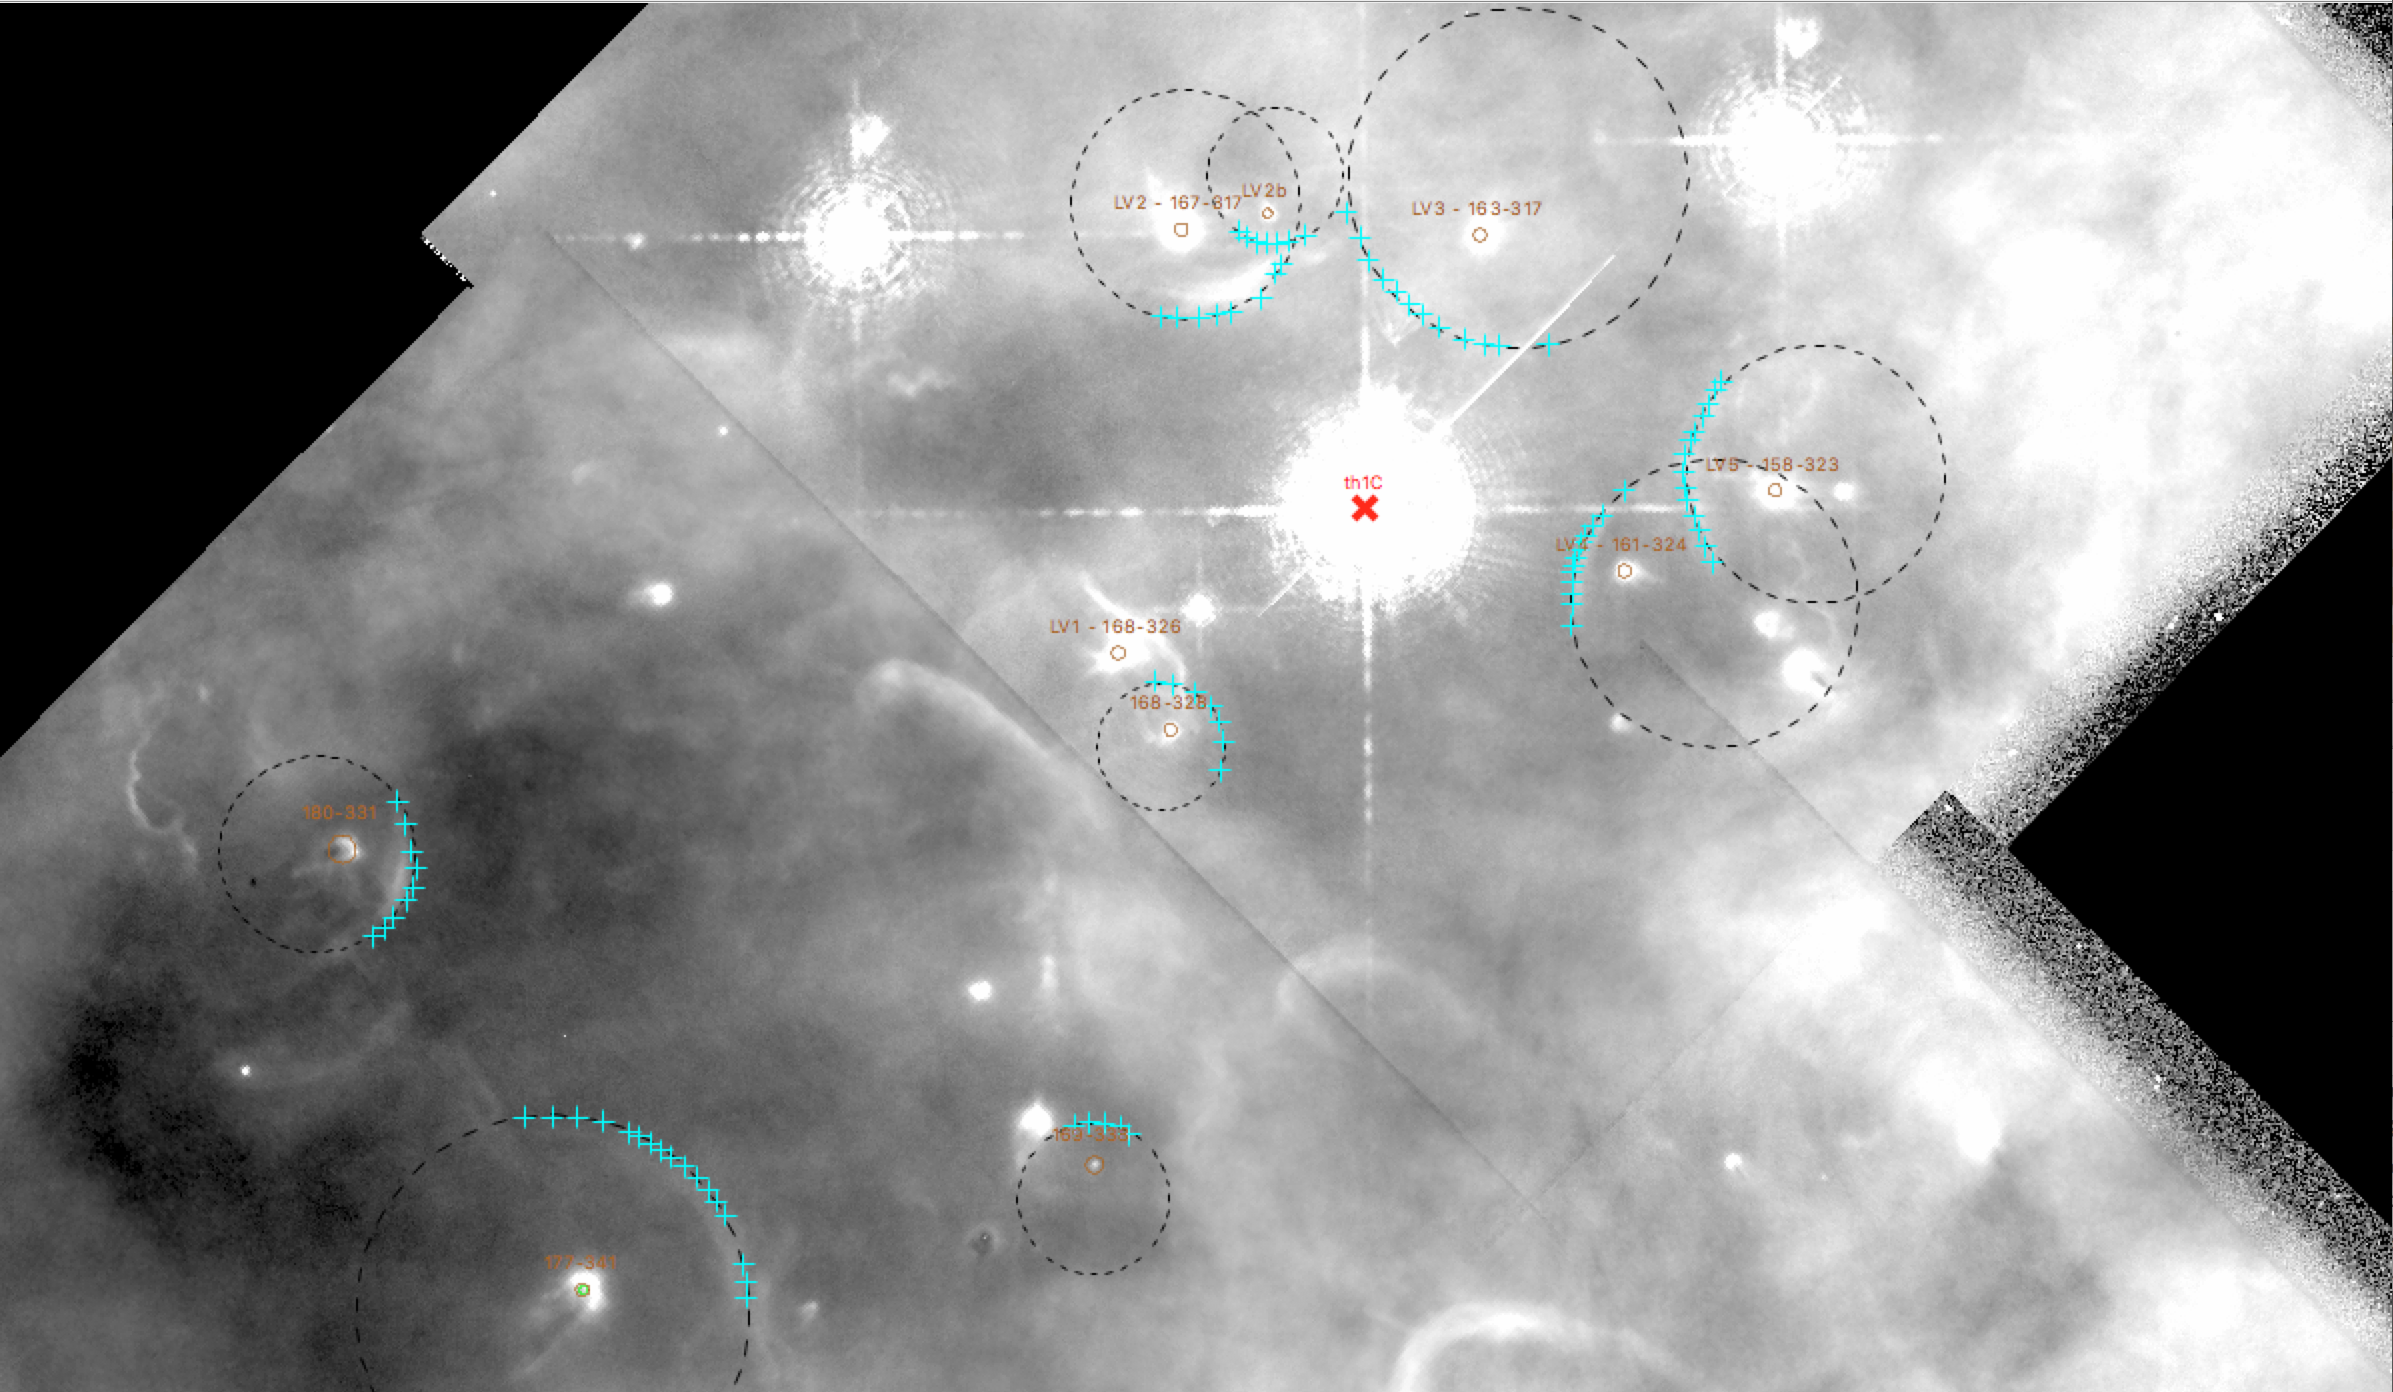
\includegraphics[width=\linewidth]{./Figures/LV-full-field-annotated}
    \caption{Imagen de la parte central de la Nebulosa de Orión donde se ubican
    los proplyds de nuestra muestra. Las cruces color cyan corresponden a las
    mediciones de la forma aparente para cada choque de proa. Los círculos
    amarillos marcan la posición de cada proplyd y la ``x'' roja corresponde a la posición de la estrella ionizante \thC{}. Los círculos negros ilustran de manera esquemática el radio de curvatura de cada choque.}
    \label{fig:proplyds-map}
\end{figure*}

\section[Metodología]{Metodología para la medición de la forma aparente.}
\label{sec:methodology}
Se utilizaron imágenes en el filtro de $[OIII]$ de la cámara WPC2 del Telescopio
Espacial Hubble (HST). Se utilizaron las herramientas del programa DS9 para
análisis de imágenes astronómicas para trazar la posición de \thC{} y de cada uno
de los proplyds de la muestra. La posición y la forma de los choques de proa fue
trazada con una serie de marcas a lo largo del choque. Las coordenadas de las marcas fueron guardadas en un archivo y luego procesadas para tener las
coordenadas del choque en el sistema de referencia del proplyd (Figura \ref{fig:proplyds-map}). El radio de curvatura aparente se obtiene haciendo un ajuste de mínimos cuadrados de la forma de un círculo de las mediciones obtenidas. $R_0$ se obtiene como la distancia mínima entre el proplyd y el ajuste circular dentro del rango de las coordenadas de las mediciones. 

\subsection{Medición de incertidumbres}

Para saber qué tan confiables son las coordenadas de las mediciones, se realizó
el procedimiento siguiente: Del total de mediciones realizadas para cada proplyd,
se crearon varias sub-muestras donde se utilizamos aproximadamente las dos terceras partes de las mediciones, pero dejando un mínimo de cuatro puntos, y se procedió a calcular los radios característicos para cada submuestra, y comprobar qué tanto se desvían estas mediciones de la original. En la figura \ref{fig:char-radii-obs} se muestran ejemplos de dichas sub-muestras para algunos proplyds.


\begin{figure*}
  \setkeys{Gin}{width=0.33\linewidth}%, trim=10 30 55 62.5}
\begin{tabular}{@{}c@{}c@{}c@{}}
 
Todos los puntos & Primera sub-muestra & Segunda sub-muestra \\ 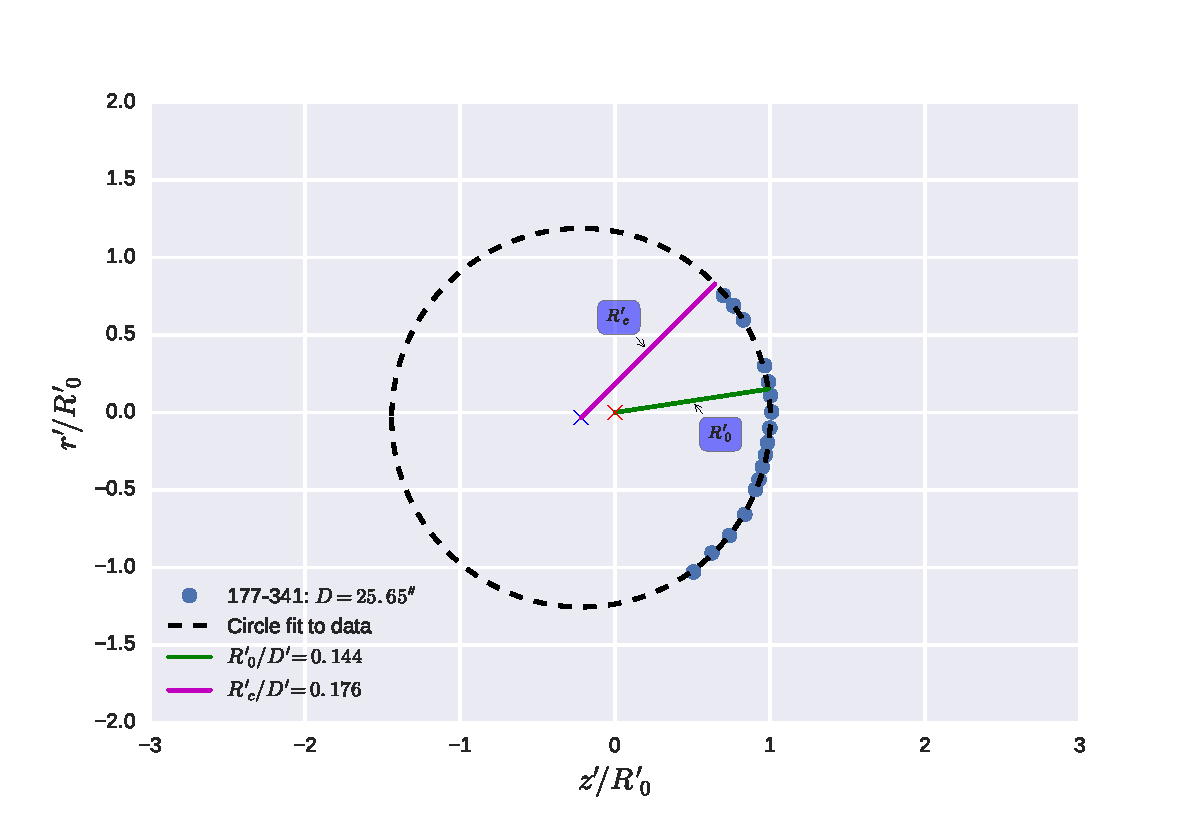
\includegraphics[clip]{./Figures/LV-bowshocks-xyfancy-positionswill-177-341} & 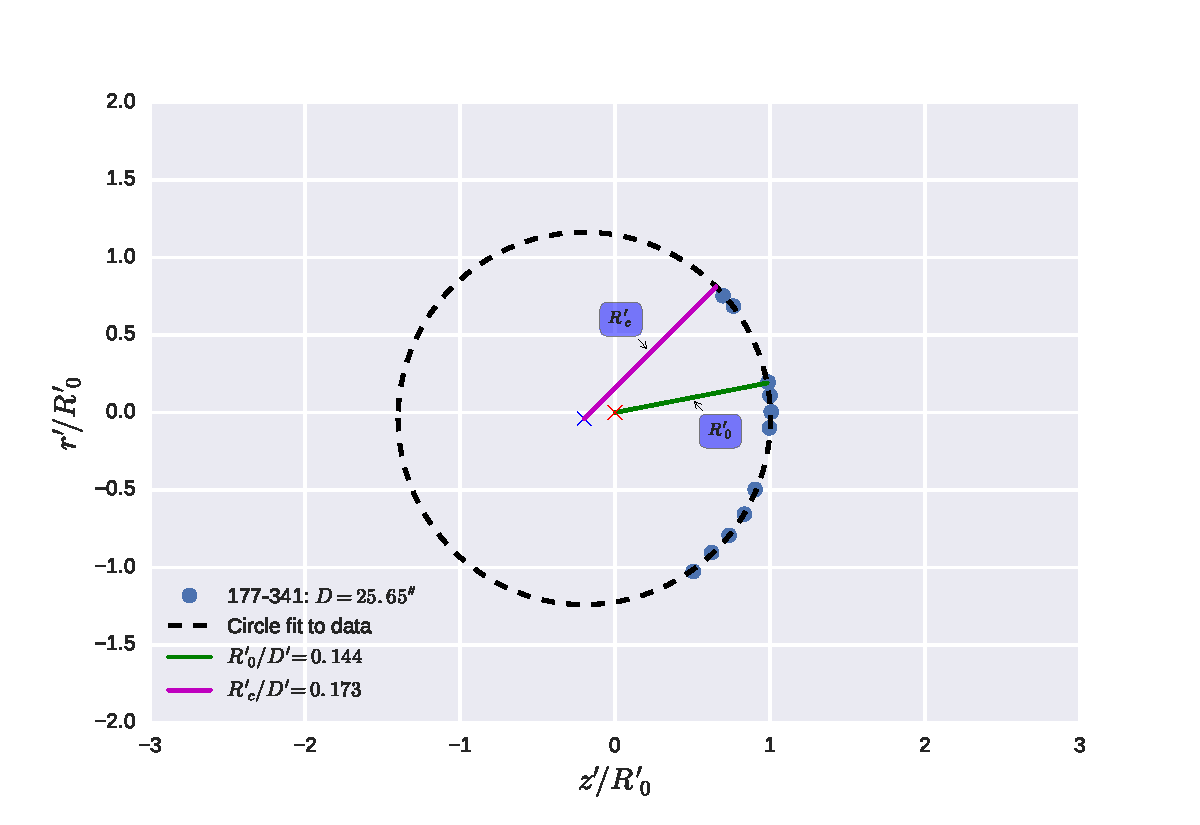
\includegraphics[clip]{./Figures/LV-bowshocks-xyfancy-positionssamp00-177-341} &
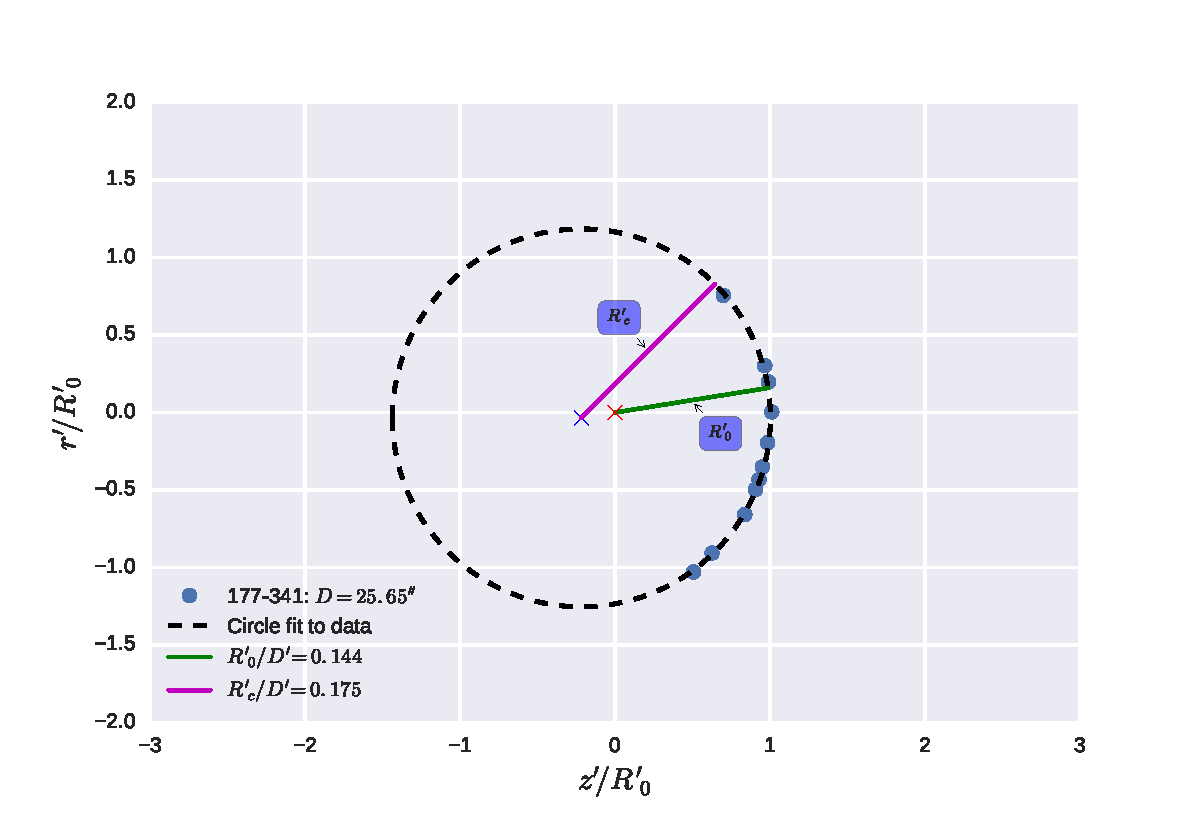
\includegraphics[clip]{./Figures/LV-bowshocks-xyfancy-positionssamp01-177-341} \\
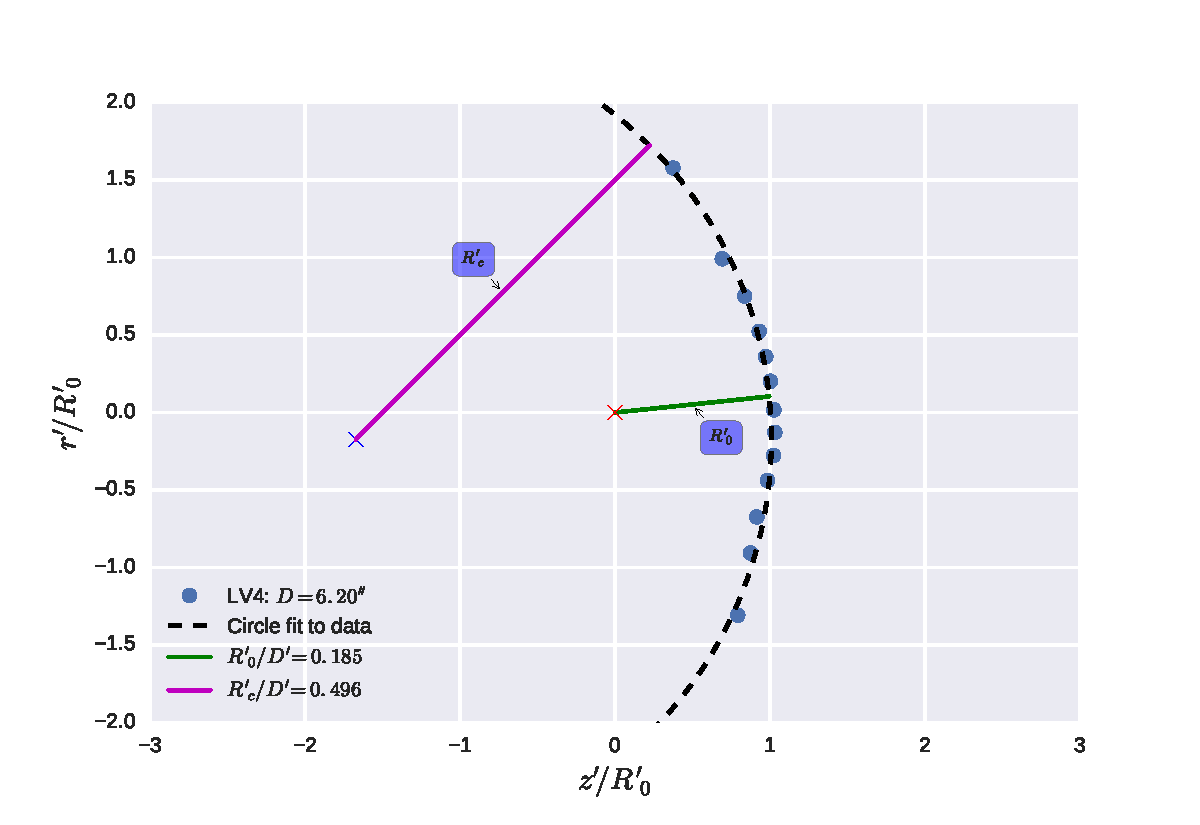
\includegraphics[clip]{./Figures/LV-bowshocks-xyfancy-positionswill-LV4} & 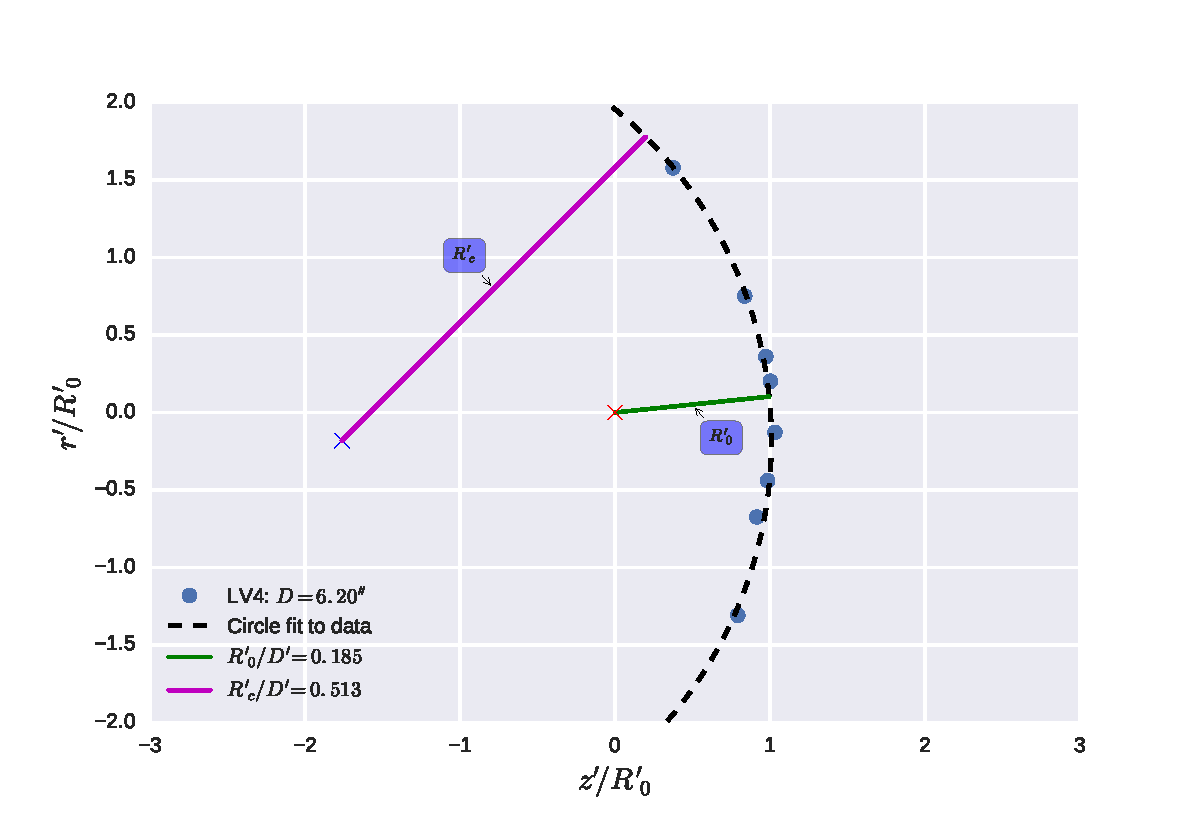
\includegraphics[clip]{./Figures/LV-bowshocks-xyfancy-positionssamp00-LV4} & 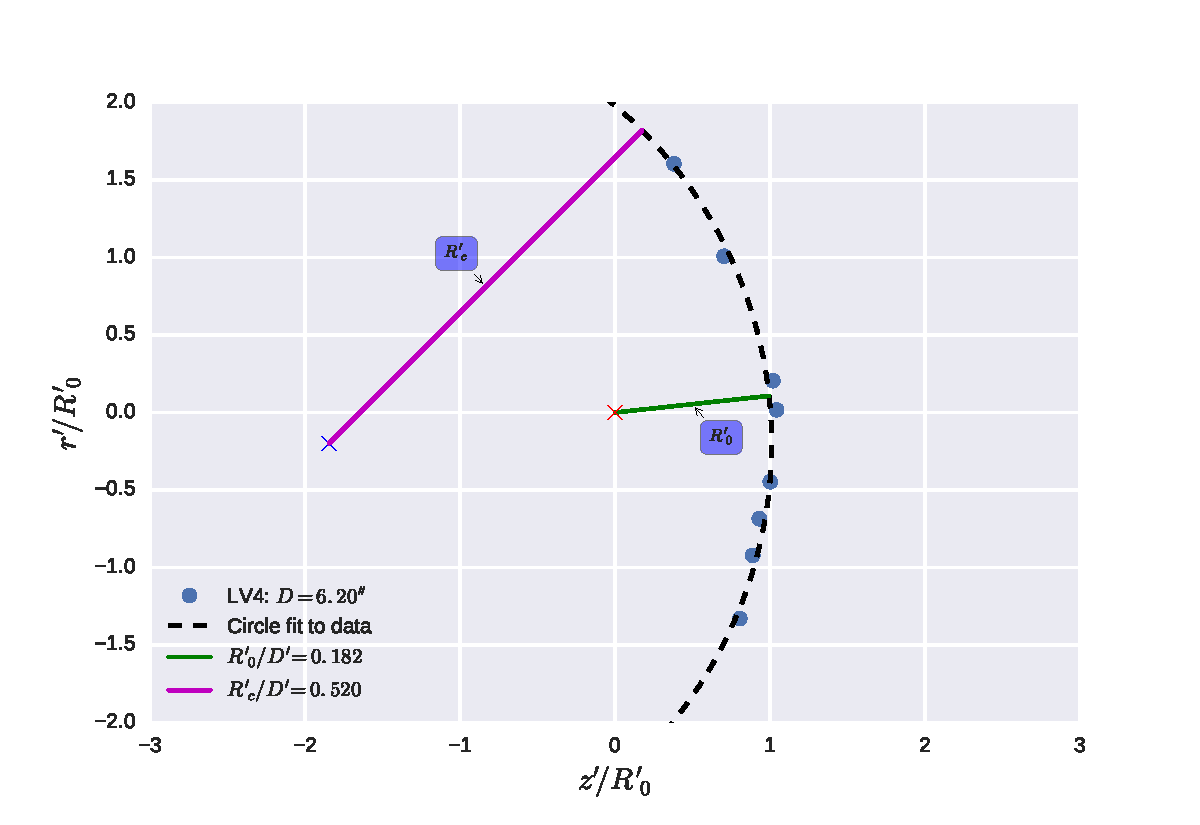
\includegraphics[clip]{./Figures/LV-bowshocks-xyfancy-positionssamp01-LV4} \\
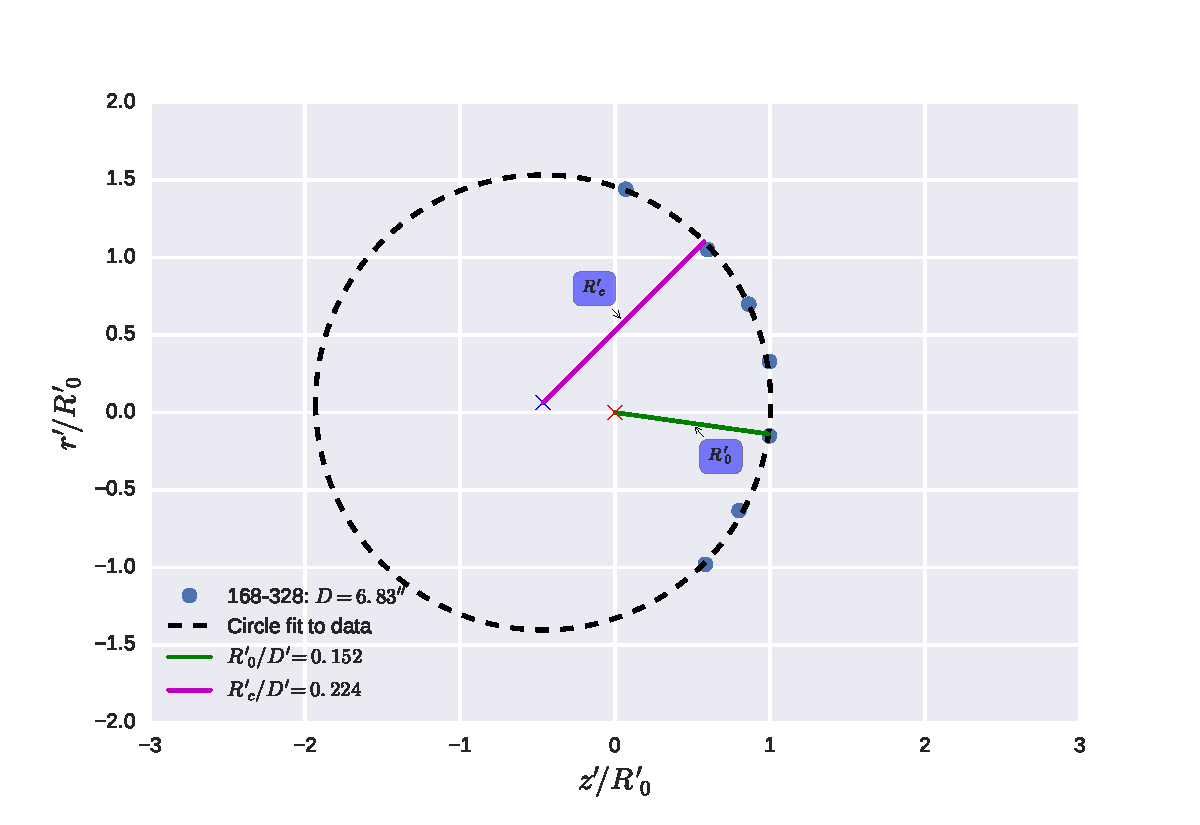
\includegraphics[clip]{./Figures/LV-bowshocks-xyfancy-positionswill-168-328} &  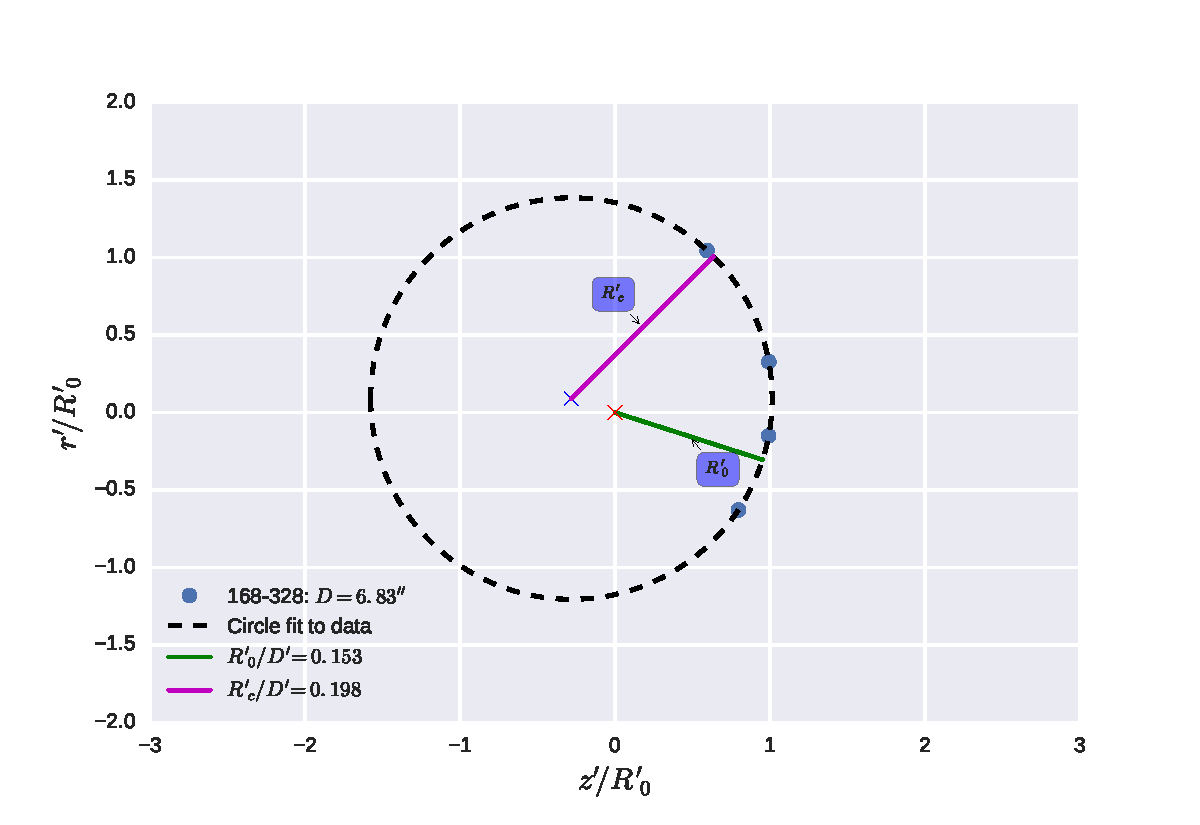
\includegraphics[clip]{./Figures/LV-bowshocks-xyfancy-positionssamp00-168-328} & 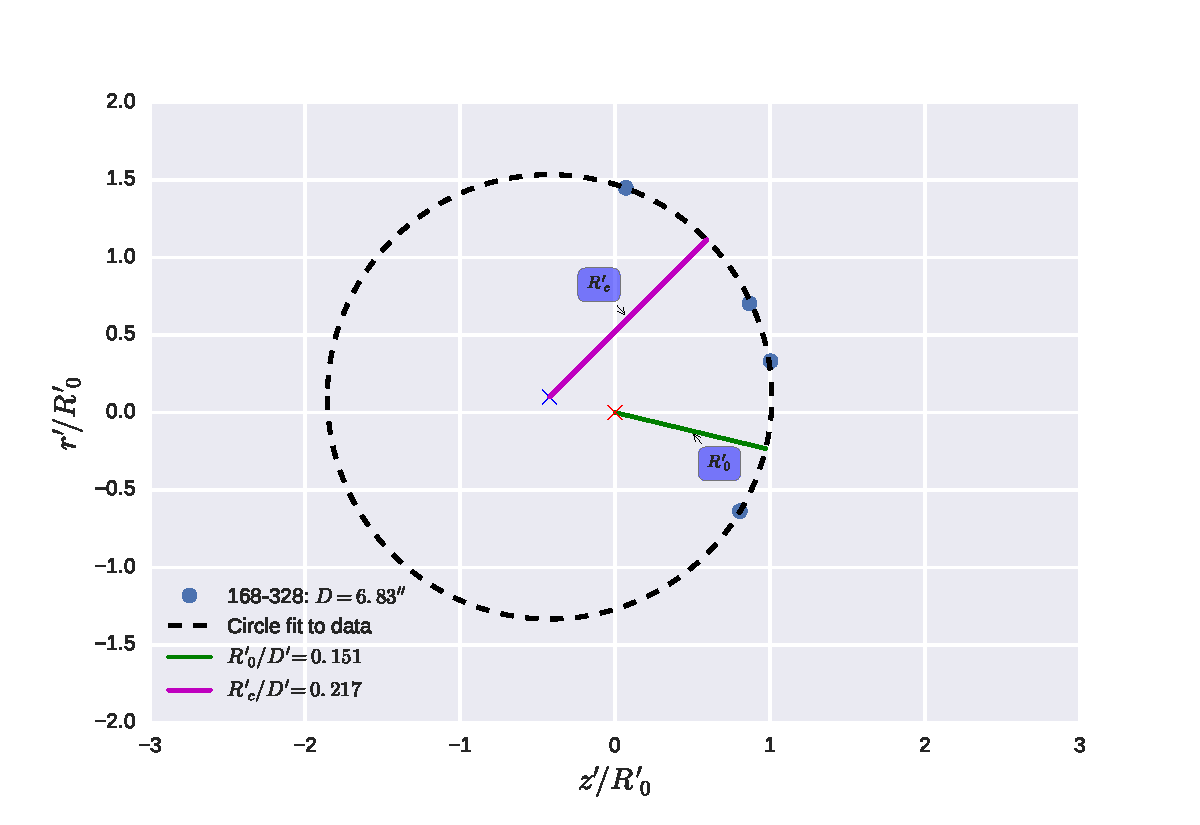
\includegraphics[clip]{./Figures/LV-bowshocks-xyfancy-positionssamp01-168-328}
\end{tabular}
\caption{Ejemplos de incertidumbres sistemáticas en los ajustes circulares a la forma de los choques para tres fuentes (desde la línea superior hasta la inferior): 177-341, LV4 y 168-328. La columna de la izquierda muestra el ajuste a todos los puntos identificados en el borde de la cáscara, donde el número y el espaciamiento de los puntos es una medida subjetiva de nuestra confianza al trazar el borde de cada cáscara. Las dos columnas restantes muestran ajustes a sub-muestras seleccionadas aleatoriamente que contienen 2/3 partes de los puntos de la muestra original para cada cáscara.}
\label{fig:char-radii-obs}
\end{figure*}

\section{Resultados}

Los radios característicos obtenidos para la muestra original y para las submuestras se muestran en la figura \ref{fig:conic-xi}. En cada pánel se utiliza un valor fijo para el parámetro de anisotropía $\xi$. Las mediciones para el proplyd LV4 son consistentes con un viento isotrópico, mientras que para los proplyds LV2b, 169-338, 180-331, 168-328, 177-341, LV3 y LV5 sus mediciones son consistentes para vientos con un grado de anisotropía bajo $(\xi \gtrsim 0.8)$. Finalmente para LV2 sus mediciones son consistentes con un viento con un grado de anisotropía alto $(\xi \lesssim 0.4)$. 

\begin{figure*}
\begin{tabular}{cc}
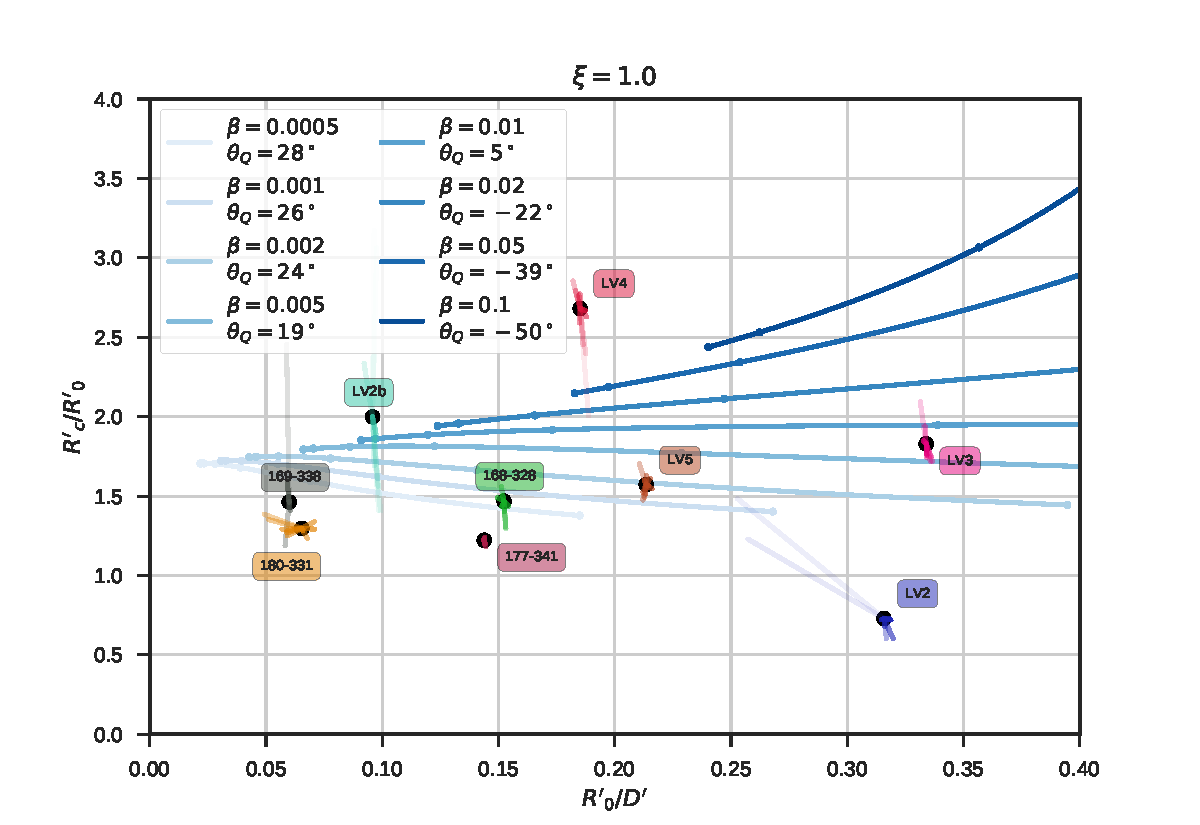
\includegraphics[width=0.48\linewidth]{./Figures/conic_xi-10} & 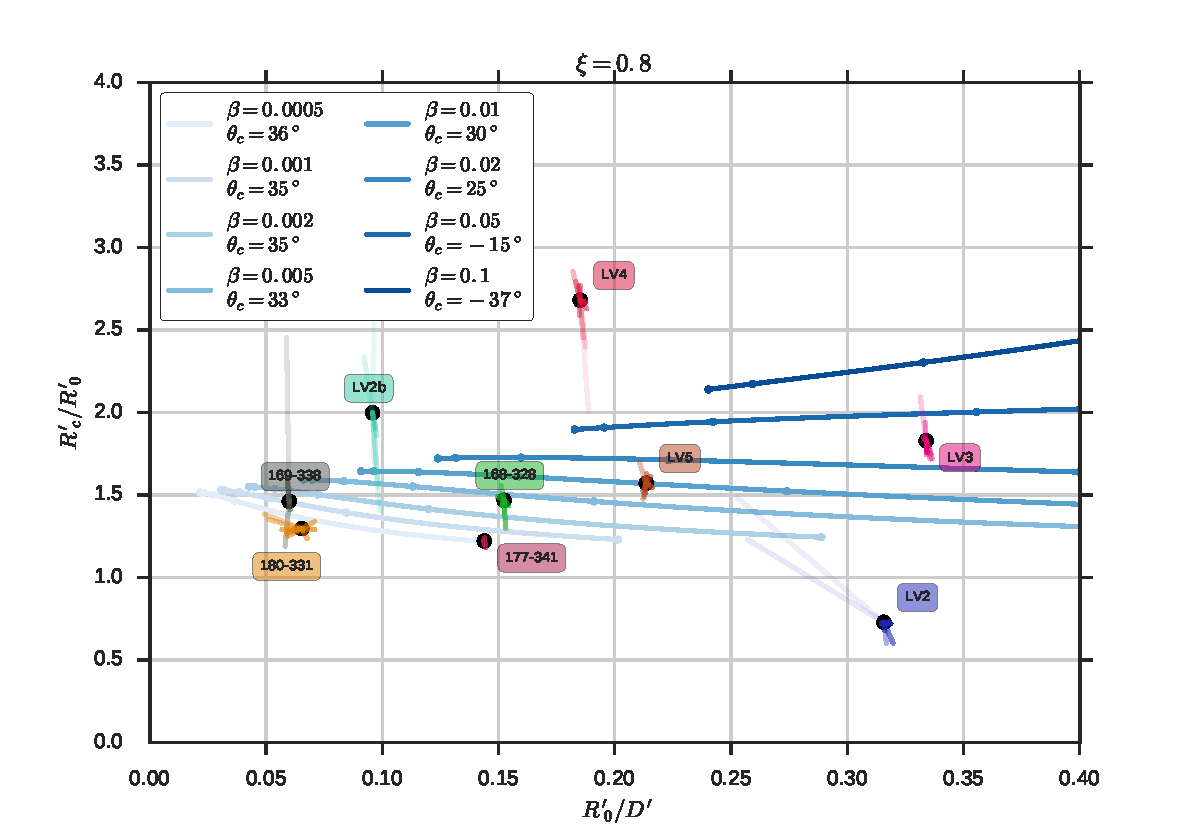
\includegraphics[width=0.48\linewidth]{./Figures/conic_xi-08} \\
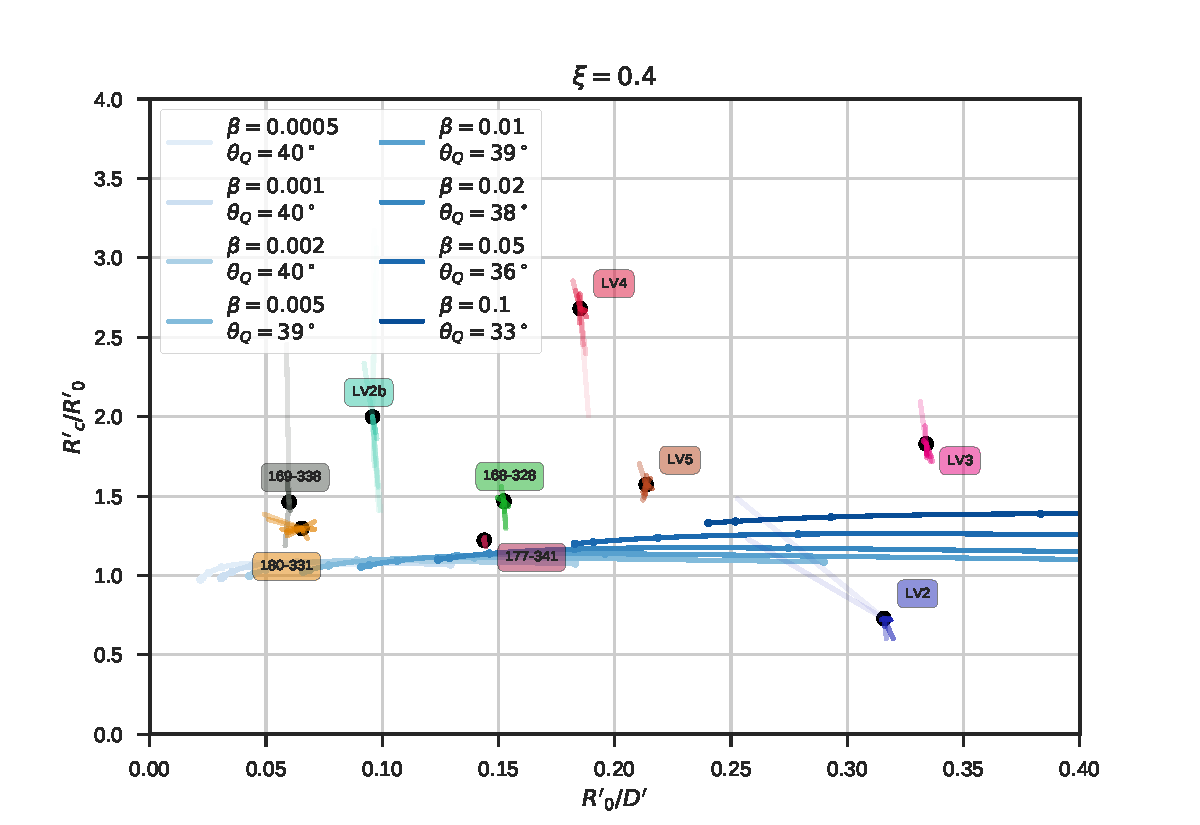
\includegraphics[width=0.48\linewidth]{./Figures/conic_xi-04} & 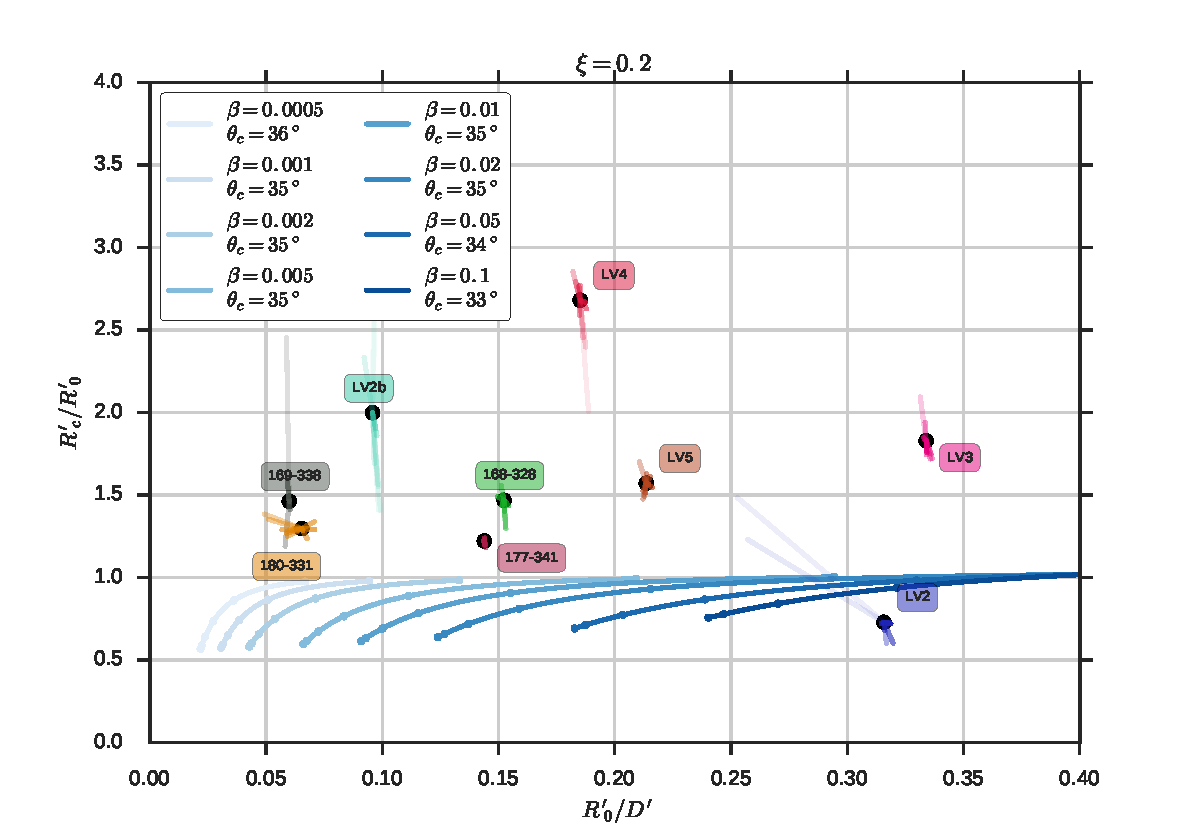
\includegraphics[width=0.48\linewidth]{./Figures/conic_xi-02} 
\end{tabular}
\caption{Mediciones de los radios característicos de los proplyds $R_c$ y $R_0$. Las curvas representan el ajuste de una cuádrica para un choque de proa con un cociente de momentos $\beta$ fijo, además se muestra su respectivo valor de $\theta_c$. Los puntos a lo largo de cada curva representan una separación en inclinación de $15^\circ$. Las mediciones para cada proplyd vienen acompañadas con el set de sub-muestras representadas como líneas radiales de colores. En cada gráfica se utiliza un valor diferente para el parámetro de anisotropía $\xi$, iniciando con un viento isotrópico $(\xi=1)$, hasta el viento  con mayor anisotropía $(\xi=0.2)$.}
\label{fig:conic-xi}
\end{figure*}

Con base a este análisis, se resume en la tabla \ref{tab:arc-fits} los ajustes a los parámteros de los proplyds: inclinación, distancia a \thC{} intrínseca $D$ y radio del choque en el eje de simetría $R_0/D$.

\begin{table*}
  \caption{Ajuste a los parámetros de los arcos para los choques de proa de los proplyds}
  \label{tab:arc-fits} 
\newcommand\C[1]{\multicolumn{1}{c}{#1}}
\begin{tabular}{llrllllrlll}\toprule
             &          & \multicolumn{3}{c}{\dotfill Obsetvado \dotfill}              & \multicolumn{6}{c}{\dotfill Ajuste teórico \dotfill} \\ 
  \C{OW}     & \C{Nombre} & \(D'\) &\C{ \(R_0'/D'\) }&\C{ \((R_c'/R_0')_{\mathrm{shape}}\) }&\C{ \((R_c'/R_0')_{\mathrm{flux}}\) }&\C{ \(\beta\) }&\C{ \(\xi\) }&\C{ \(|i|\) }&\C{ \(D\) }&\C{ \(R_0/D\)}\\
  \C{(1)}& \C{ (2) }&\C{ (3)    }&\C{    (4)      }&\C{              (5)           }&\C{           (6)             }&\C{     (7)   }&\C{   (8)   }&\C{   (9) }&\C{  (10) }&\C{   (11)} \\
\midrule     
 168-328  &            &    6.8  &  $0.152 \pm 0.001$  &  $1.42 \pm 0.09$   &  $1.45 \pm 0.05$     &  $0.018 \pm 0.003$  &  0.4 -- 0.6  &  $33 \pm 3$   &  $0.017 \pm 0.001$  &  $0.115 \pm 0.005$  \\
 169-338  &            &  16.4  &  $0.059 \pm 0.001$  &  $1.76 \pm 0.48$   &  $1.50 \pm 0.05$     &  $0.002 \pm 0.001$  &  0.8 -- 0.8  &  $43 \pm 8$   &  $0.049 \pm 0.006$  &  $0.035 \pm 0.005$  \\
 177-341  & HST1   & 25.6  &  $0.144 \pm 0.001$  &  $1.21 \pm 0.02$   &  $1.25 \pm 0.02$     &  $0.018 \pm 0.003$  &  0.1 -- 0.2  &  $30 \pm 5$   &  $0.064 \pm 0.003$  &  $0.115 \pm 0.005$  \\
 180-331  &             &  25.1  &  $0.061 \pm 0.007$  &  $1.30 \pm 0.05$   &  $1.27 \pm 0.05$     &  $0.003 \pm 0.001$  &  0.4 -- 0.4  &  $35 \pm 7$   &  $0.066 \pm 0.007$  &  $0.047 \pm 0.005$  \\
 167-317  &  LV2     &    7.8  &  $0.305 \pm 0.025$  &  $0.81 \pm 0.28$   &  $1.50 \pm 0.1$      &  $0.085 \pm 0.015$  &  0.1 -- 0.2  &  $13 \pm 13$  &  $0.017 \pm 0.001$  &  $0.225 \pm 0.005$  \\
               & LV2b    &   7.2  &  $0.097 \pm 0.002$  &  $2.00 \pm 0.62$   &  $1.63 \pm 0.08$     &  $0.008 \pm 0.003$  &  0.8 -- 0.8  &  $28 \pm 13$  &  $0.018 \pm 0.002$  &  $0.078 \pm 0.013$  \\
 163-317  & LV3      &   6.9  &  $0.334 \pm 0.002$  &  $1.81 \pm 0.12$   &  $1.85 \pm 0.15$     &  $0.075 \pm 0.025$  &  0.6 -- 0.8  &  $35 \pm 5$   &  $0.018 \pm 0.001$  &  $0.205 \pm 0.025$  \\
 161-324  & LV4      &   6.2  &  $0.186 \pm 0.002$  &  $2.59 \pm 0.24$   &  $2.05 \pm 0.07$     &  $0.040 \pm 0.014$  &  0.8 -- 1.0  &  $18 \pm 12$  &  $0.014 \pm 0.001$  &  $0.160 \pm 0.028$  \\
 168-323  & LV5      &   9.6  &  $0.213 \pm 0.002$  &  $1.57 \pm 0.07$   &  $1.60 \pm 0.07$     &  $0.055 \pm 0.005$  &  0.2 -- 0.4  &  $20 \pm 5$   &  $0.022 \pm 0.001$  &  $0.190 \pm 0.010$  \\
\bottomrule
\end{tabular}
\begin{minipage}{0.95\linewidth}
  Notes --
%
  Col.~(1): ID de la fuente \citep{ODell:1994a}.
%
  Col.~(2): Nombre alternativo de la fuente.
% 
  Col.~(3): Distancia proyectada desde \thC{}, segundos de arco.
%
  Col.~(4): Radio exterior aparente a lo largo del eje, normalizado con la distancia proyectada, con una incertidumbre de \(\pm 1\sigma\), determinado con el ajuste circular decrito en \S~\ref{sec:methodology}.
% 
  Col.~(5): Radio de curvatura aparente, normalizado con el radio a lo largo del eje, con incertidumbres de \(\pm 1\sigma\), determinado con el ajuste circular descrito en \S~\ref{sec:methodology}.
% 
  Col.~(6): Igual que Col.~(5) pero aplicando el criterio adicional de que el brillo superficial del proplyd obtenido debe coincidir con la predicción teórica.
%
  Col.~(7): Cociente de momentos entre el viento del proplyd y la estrella O (ver capítulo \ref{chap:hipersonica}). 
% 
  Col.~(8): Parámetro de anisotropía del viento del proplyd.
% 
  Col.~(9): Inclinación respecto al plano del cielo, en grados.
% 
  Col.~(10): Distancia real desde \thC{}, parsecs.
%
  Col.~(11): Radio real de la cáscara a lo largo del eje, normalizado con distancia.

\end{minipage}
\end{table*}

\chapter{Conclusiones}
This is chapter 6

\bibliographystyle{mnras}
\bibliography{orion_tesis}

\end{document}
